\documentclass[11pt]{book}
\usepackage[top=3cm,bottom=3cm,left=3.2cm,right=3.2cm,headsep=10pt,a4paper]{geometry}

\usepackage{parskip}
\usepackage{enumerate}
\usepackage{enumitem}
\usepackage{graphicx}
\usepackage{float}
\usepackage{hyperref}
\usepackage{rotating}
\setlength\parindent{0pt}
\usepackage{setspace}
\setcounter{tocdepth}{2}
\setcounter{secnumdepth}{2}

\usepackage{xcolor}
\usepackage{avant}
\usepackage{microtype}
\usepackage{listings}
\usepackage[utf8]{inputenc}

\usepackage{titlesec}

\titlespacing\section{0pt}{12pt plus 4pt minus 2pt}{0pt plus 2pt minus 2pt}
\titlespacing\subsection{0pt}{12pt plus 4pt minus 2pt}{0pt plus 2pt minus 2pt}
\titlespacing\subsubsection{0pt}{12pt plus 4pt minus 2pt}{0pt plus 2pt minus 2pt}

\bibliographystyle{vancouver}

\begin{document}

\frontmatter

\begin{titlepage}
	
	\begin{center}
		
		% \textbf{\textsc{\Large Norwegian University of Science and Technology}}
		% \\[1.5cm]
		
		\textsc{\Large TDT4290 Customer Driven Project}
		\\[1.5cm]
		
		\rule{\linewidth}{0.5mm}
		\\[1cm]
		
		\textbf{\LARGE Virtual Walls - Walls that tell us stories}
		\\[1cm]
		
		\rule{\linewidth}{0.5mm}
		\\[1.5cm]
		
		\Large{  \today}
		\\[1.5cm]
		
		\textsc{\Large Group 2}
		\\[0.5cm]
		
		\Large
		{
			Odd Fredrik Rogstad \\
			Christian Frøystad \\
			Simon Stastny \\
			Knut Nergård
		}
		\\[2cm]
		
		
		\begin{figure}[hb]
			\begin{minipage}[b]{0.45\linewidth}
				\centering
				
\includegraphics[width=\textwidth]{images/ntnu_logo}
			\end{minipage}
			\hspace{0.5cm}
			\begin{minipage}[b]{0.45\linewidth}
				\centering
				
\includegraphics[width=\textwidth]{images/sintef}
			\end{minipage}
		\end{figure}
		\begin{figure}[hb]
			\begin{minipage}[b]{0.45\linewidth}
				\centering
				
\includegraphics[width=\textwidth]{images/tagcloud}
			\end{minipage}
			\hspace{0.5cm}
			\begin{minipage}[b]{0.35\linewidth}
				\centering
				
\includegraphics[width=\textwidth]{images/stfk}
			\end{minipage}
		\end{figure}
		\vfill
		%\vfill 
		
	\end{center}
		
\end{titlepage}



\chapter{Abstract}
\begin{quotation}
The assignment relates to the EU-IST project TAG CLOUD. TAG CLOUD will develop innovative digital solutions with the aim to increase the engagement of people in culture and cultural heritage. The main aspects that will be investigated are: new interaction interfaces with cultural artefacts, user as a contributor and personalized information. In Norway, the focus is “culture in the landscape”, i.e. the discovery of cultural memories that we meet when walking around in cities, in villages and in the nature.  \cite[p. 47]{compendium}
\end{quotation}

The aim of this particular project is to develop a concept and a prototype that will make information about cultural heritage more accessible and fun! This will be accomplished by creating a mobile application that lets users consume content from cultural databases in an exploratory format.



\tableofcontents
\listoffigures
\listoftables

\mainmatter
\chapter{Introduction}
This report describes the planning and execution of the project ``Virtual Walls - Walls that tell us stories'' (later in this report only referred to as Virtual Walls or the system) on behalf of eTrøndelag and Sintef ICT.

The aim of the project is to communicate and engage people in cultural heritage. The assigned project is part of the course TDT4290 - Customer driven project at NTNU, and also an ongoing project at Sintef ICT on behalf of eTrøndelag and the EU initiated project TAG-CLOUD.

Today most places of cultural or historical significance is mapped and has a rather large amount of connected data. This information might be hard to gain access to, written in a form more suited for scholars than the average man, or simply not written down at all.

The system will help the user discover, consume and share information about places, buildings, persons, events, and other historically significant information. The user can add new information, improve existing information, comment on information or walls, make new walls and share a wall on social media.

Both the walls and the information will be categorized using taxonomy so that the user might filter the sort of information he is looking for.

The goal of the project is to make information about cultural heritage more accessible, understandable and fun for the common man.

\chapter{Project plan}
This chapter will give an overview of how the work is to be structured and the most important milestones.

\section{Project directive}
The project directive describes the background and mandate of the project.

\subsection{Project name}
The customer has given the project the name ``Virtual Walls - walls that tells us stories''. The project will, in this report, be referred to as ``Virtual Walls'' or the system. The name is derived from ``Væggen'' in Copenhagen which was the inspiration of this project.

\subsection{Project sponsor}
The sponsor of the project is eTrøndelag together with SINTEF ICT.
eTrøndelag is the division at Sør-Trøndelag county that focuses on ICT. Their responsibility lies in ICT strategy, digital communication and cooperation, infrastructure and digital cultural development. The division has four advisors.

SINTEF ICT is the ICT unit at SINTEF, which is the largest independent research organization in Scandinavia. SINTEF is a non-commercial organization which means that all the profits goes into new research, equipment and development of staff. The organization has about 2100 employees.

\subsection{Partners}
\subsubsection{Customer}
Name: Eistein Guldseth\\
Role: Advisor Digital communication and Interaction, STFK\\
Mobile: +47 414 74 826\\
E-mail: eistein.guldseth@stfk.no

Name: Jacqueline Floch\\
Role: Senior scientist at SINTEF ICT\\
Mobile: +47 930 08 536\\
Fax: +47 73 59 43 02\\
E-mail: jacqueline.floch@sintef.no

\subsubsection{Advisor}
Name: Reidar Conradi\\
Role: Professor, NTNU\\
Mobile: +47 91 89 70 29\\
Phone: +47 73 59 34 44\\
E-mail: conradi@idi.ntnu.no

\subsubsection{Group}
Name: Odd Fredrik Rogstad\\
Mobile: +47 99 10 73 27\\
E-mail: oddfredrikrogstad@gmail.com

Name: Christian Frøystad\\
Mobile: +47 45 21 70 66\\
E-mail: chrisfro@stud.ntnu.no

Name: Simon Stastny\\
Mobile: +47 45 16 62 98\\
E-mail: simonst@stud.ntnu.no

Name: Knut Nergård\\
Mobile: +47 41 25 67 20\\
E-mail: knut.nerga@gmail.com

\subsection{Background for the project}
Today, if you want information about cultural heritage you will have to access many different sources, and the information might be less than accessible. The joint European project TAG CLOUD wishes to change this, and also bring together content provided by experts and individuals. TAG CLOUD is to develop innovative digital solutions to engage people in cultural heritage by making the information more accessible and involving the user in the content production.

In connection with this project eTrøndelag has decided, together with SINTEF ICT, to explore the possibility of using Virtual Walls to spread information about cultural heritage in Trondheim.

During the last 5 - 6 years, smart phones has become more and more common. In the later years mobile Internet has also become somewhat common. This has made this project possible, as the users do not need to carry an ordinary computer around.

\subsection{Project goal}
The goal of the project is producing a prototype of the system that might be experimented with and tested in different contexts. The prototype should be accompanied by excellent documentation, both for users and developers.

\section{Tools}
This section describes the tools used to communicate, develop and implement the system.

\subsection{Hardware}

\subsection{Software}

\subsection{Collaboration and communication}
This section describes the tools used to collaborate and communicate throughout the project.

\subsubsection{Google Docs}
Google docs is a freeware web-based office suite that enables multiple members to collaborate on documents, spreadsheets, presentations, drawings etc. from any computer with Internet access. Google docs uses Google Drive, which is a file storage and synchronization service. That means that two or more persons can work on the same document simultaneously, at different geographical places. 

We chose to use Google Docs because everyone already had used this with great success on previous projects. It is also fairly simple to use, so no training were needed. Since Google Docs has some limitations regarding appearance and navigation in documents, we used \LaTeX~to produce the final document.

\subsubsection{\LaTeX}
\LaTeX~is a document markup language and document preparation system for the \TeX~typesetting program. \LaTeX~enables us to make large, professional looking documents without all the hassle regarding table of content, placing of pictures and diagrams, cross-references, making tables etc.. 

Some group members had some experience with the language, but everyone else was eager to learn and try it out.

\subsubsection{Dropbox}
Is a file hosting service that offers cloud storage and file synchronization, much like Google Drive. We only used Dropbox as an collaboration tool with the customer, as in sharing files, etc.. We found that Google Drive, with the possibility to use the embedded office suite, Google Docs, were the best alternative as an collaboration tool for document writing.

\subsubsection{Facebook}
Facebook is an online social networking service used by 1 110 million users worldwide [investor.fb.com/releasedetail.cfm?ReleaseID=761090]. We started a private group, ``TDT4290 - CDP - Virtual Wall'', and used this to everything from planning meetings, having scrum stand ups to discuss about the project. 

At first we had some problems with time-sensitive matters, such as revoking meetings, where some did not see the revoking post on facebook. Therefore we started using email for such matters.

\subsubsection{Email}
Email were used for communicating with both the customer and advisor. Within the group it was used for time sensitive matters.

\subsubsection{GitHub}
GitHub is a web-based hosting service for software development project that use the Git revision control system, which is a distributed revision control tool (DRCS). Since Git is distributed every developer has their own local repository, independent of the centralized repository, that allows developer to work in offline mode and each of the local repositories acts as a backup. This was used during the implementation of the system.

Everyone had used GitHub on other projects, but almost every member needed a refresher

\subsubsection{Trello}
Trello is a free web-based project management application that uses the paradigm kanaban. Kanaban, a Japanese word that roughly mens ``card'' or ``signboard'', is a method made famous by the car manufacturer Toyota in the 1980s for supply management. 

Kanaban is fairly simple, a project is represented by a board, the board contains lists, that corresponds to a workflow. Lists contains cards that represents tasks.

\begin{figure}[H]
      \centering
      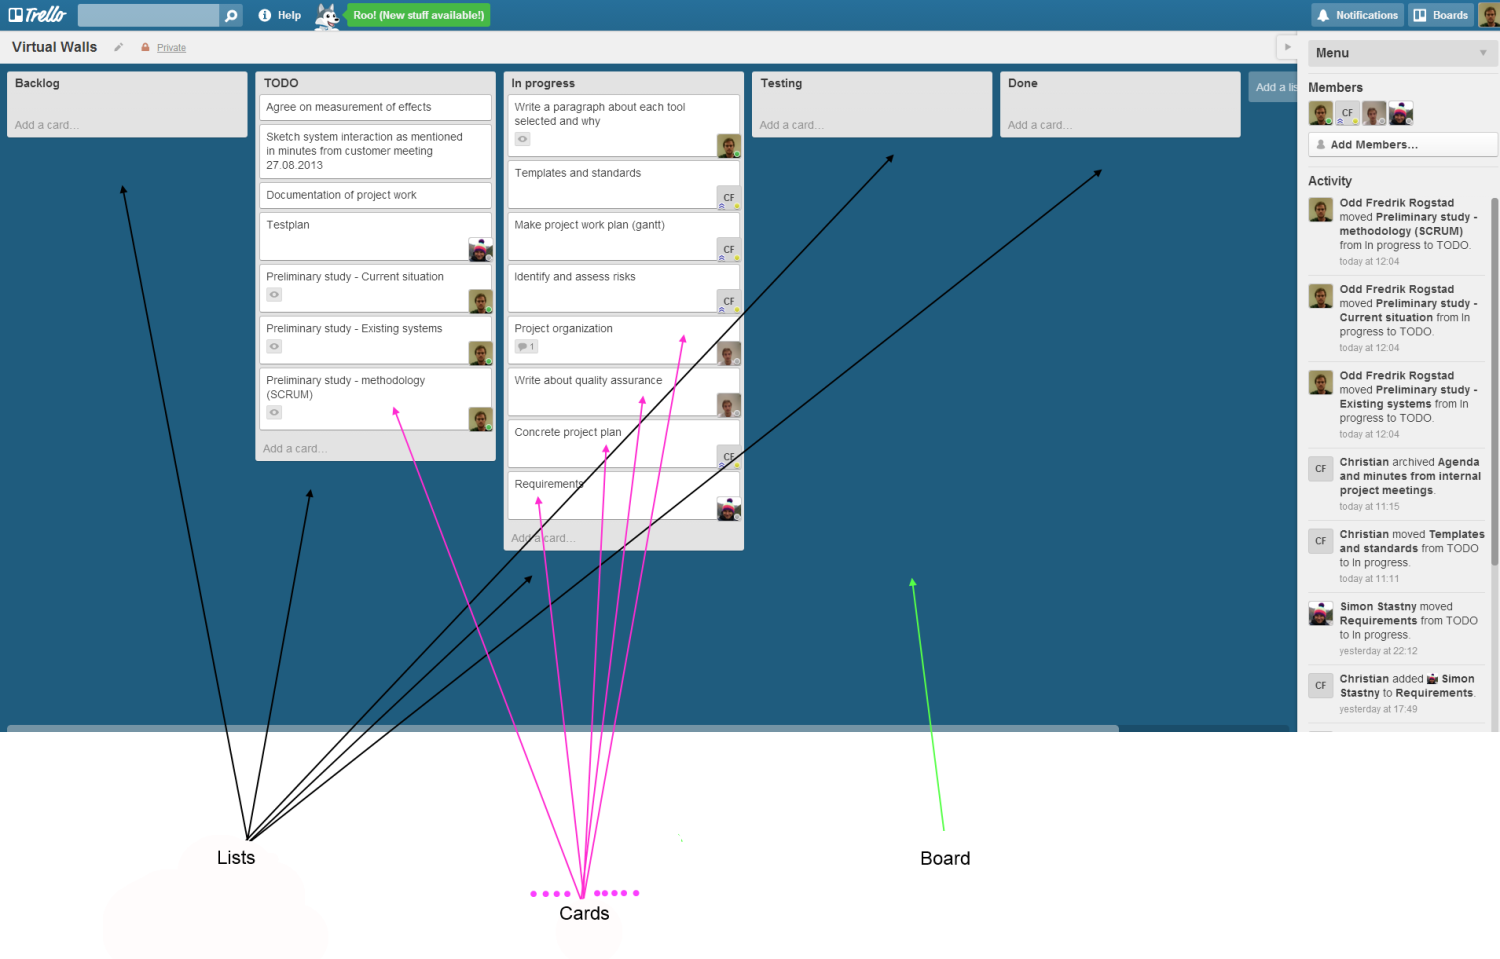
\includegraphics[width=0.8\textwidth]{Figures/trello.png}
      \caption{Screenshot of Trello}
      \label{fig:tools_trello}
\end{figure}

Figure~\ref{fig:tools_trello} shows how we used it for document work. There are several lists; ``TODO'', ``In Progress'', ``Testing'' and ``Done'', which represents the workflow. We started by populating the ``TODO''-list, with all the appendices that were needed. Then we divided the different tasks between the group members, and started working. When a person worked on a task, then the corresponding card would be in the ``In progress'' list, when the task were finished, it was moved to the ``Testing'' list, for quality assurance. If it was approved, it was moved to ``Done'' list, if not, back in the ``In Progress'' list.

\subsection{Allocated time}
The course the project is part of amounts to 15 points of credit, which indicates that each member of the group should work for about 25 hours on the project each week. Given that the group consists of 4 members, and that the project run over 13 weeks, we get a total of allocated time that amounts to 25 x 4 x 13 = 1300 hours.

Due to the diversity of the group, one in a full time job, the others attending different classes, the group has few meetings in person each week. As such, every group member is free to plan his own work each week, but has to meet at the weekly group meeting. As a result of this the group has only a few items on its weekly agenda: internal group meeting, meeting with advisor and meeting with customer.

\section{Detailed plan}
The goal of this chapter is to indicate how the project was executed. It was written as a guide on beforehand, but has been revised during the project lifetime in order to provide a better level of detail.

\subsection{Phases}
Here follows a short summary of the contents, duration and expected outcome of each phase.

\subsubsection{Planning and preliminary study}
Duration: 21.08.2013 - 11.09.2013\\
Expected outcome: Preliminary first chapters of report, requirements and test plan.

\subsubsection{Sprint 1}
Duration: 11.09.2013 - 25.09.2013\\
Expected outcome: Architectural documentation, refined requirements and test plan, and minimal working prototype. Complete phase document.

\subsubsection{Sprint 2}
Duration: 25.09.2013 - 09.10.2013\\
Expected outcome: Refined requirements and test plan, working prototype with developer documentation. Also complete phase document

\subsubsection{Sprint 3}
Duration: 09.10.2013 - 23.10.2013\\
Expected outcome: Refined requirements and test plan, working prototype with even better and more complete developer documentation. Complete phase document.

\subsubsection{Sprint 4}
Duration: 23.10.2013 - 06.10.2013\\
Expected outcome: Refined requirements and test plan, working prototype with excellent developer documentation.

\subsubsection{Finalization}
Duration: 06.11.2013 - 21.11.2013\\
Expected outcome: Excellent project report, presentation and prototype accompanied by user and developer documentation. Phase focuses primarily on finishing report and presentation, but also polishing the documentation.

\subsection{Activities}
Every week some repeating meetings will take place.

\subsubsection{Customer meeting}
Each week a status is given to the customer, as well as clarifying anything being unclear at that time. Backlog is prioritized every second week before the start of the next sprint.

\subsubsection{Advisor meeting}
This meeting is to report status and get valuable feedback and advice from the advisor.

\subsubsection{Internal group meeting}
Since it is not possible for the group to work together during normal work hours, this internal group meeting serves as the planning meeting for the coming week.

\subsection{Milestones}

\subsubsection{Pre-delivery of report}
Due: 14.10.2013 (08.10.2013 electronically to advisor)\\
Delivery of the chapters Abstract, Introduction, Pre-study and the one containing choice of development model. The outline of the report should also be finalized in the table of contents. The outline does not need to be complete, but should give a good indication as to what each sections is to discuss.

\subsubsection{Production of reports}
Due: 20.11.2013\\
The report is to be copied and bound in four copies no later than 20.11.2013. Preferably earlier.

\subsubsection{Final delivery and presentation}
Due: 21.11.2013\\
Presentation for customer, advisor and censor. After the presentation, a copy of the report should be given to the customer and three copies should be delivered to the information desk at IDI. A PDF version should also be sent by email to anreala@idi.ntnu.no.

All copies is to be accompanied with a CD that contain the implementation, documentation and a PDF version of the report. The content of this CD will be documented with a ``Readme.txt'' file, as specified in the compendium.

\subsection{Gantt diagram}
\begin{figure}[H]
      \centering
      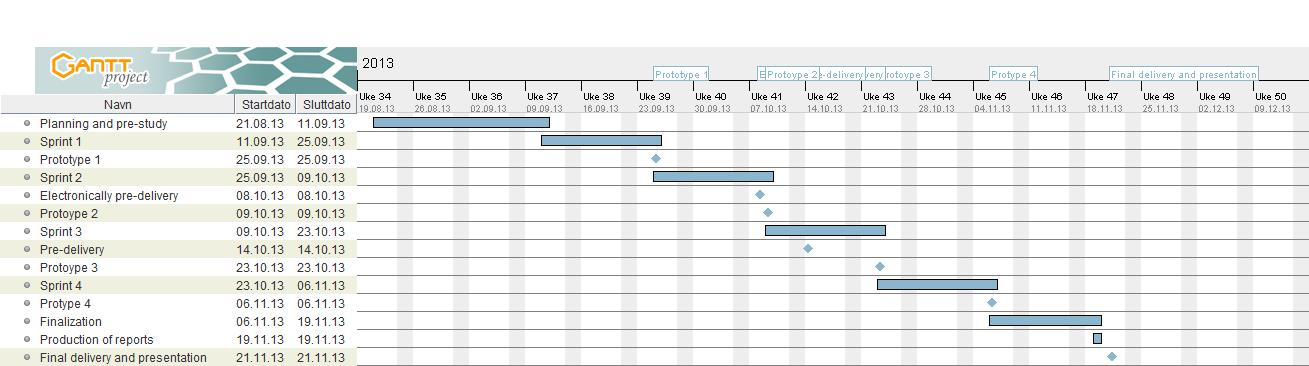
\includegraphics[width=1.0\textwidth]{Figures/gantt.jpg}
      \caption{Overview of project}
      \label{fig:plan_gantt}
\end{figure}

\begin{table}[H]
\centering
\begin{tabular}{ l | l l l l l l }
	Activity		Planning 	& Sprint 1 	& Sprint 2 	& Sprint 3 	& Sprint 4 	& Finalization	\\ \hline		
	Lectures		& 60 		& 4 		& 4 		& 4 		& 4 		& 4				\\ \hline
	Admin			& 25 		& 20 		& 20 		& 20 		& 20 		& 50			\\ \hline
	Planning		& 50 		& 8 		& 8 		& 8 		& 8 		& 50			\\ \hline
	Pre-Study		& 100 		& 20 		& 20 		& 10 		& 10 		& 10			\\ \hline
	Requirements	& 60 		& 15 		& 15 		& 10 		& 10 		& 0				\\ \hline
	Design			& 5 		& 30 		& 30 		& 15 		& 15 		& 0				\\ \hline
	Implementation	& 0 		& 60 		& 60 		& 50 		& 50 		& 10			\\ \hline
	Testing			& 0 		& 22 		& 22 		& 50 		& 50 		& 38			\\ \hline
	Documentation	& 0 		& 21 		& 21 		& 33 		& 33 		& 38			\\ \hline
	Sum				& 300 		& 200 		& 200 		& 200 		& 200 		& 200
\end{tabular}
\label{tab:plan_time_per_phase}
\caption{Time sheet per phase}
\end{table}

\section{Risks}\label{sec:project_risk_assessment}

\begin{table}[H]
\centering
\begin{tabular}{ l  p{11cm} }
	Nr						& R1 																		\\ \hline
	Activity				& All 																		\\ \hline
	Risk factor				& Group member having a full time job in addition to being 75 \% student 	\\ \hline
	Consequences			& H: The quality and scope of the project might suffer 						\\ \hline
	Probability				& M 																		\\ \hline
	Strategy and actions	& Monitor situation closely. Have clear assignments and deals 				\\ \hline
	Deadline				& Continuously 																\\ \hline
	Responsible				& Project leader 															\\ 
\end{tabular}
\label{tab:risk_1}
\caption{R1}
\end{table}

\begin{table}[H]
\centering
\begin{tabular}{ l  p{11cm} }
	Nr						& R2 																		\\ \hline
	Activity				& All 																		\\ \hline
	Risk factor				& Disease 																	\\ \hline
	Consequences			& H: The available work power might be reduced and tasks delayed. 			\\ \hline
	Probability				& M 																		\\ \hline
	Strategy and actions	& All tasks to be entered into task management system. 
							  When sick, the group should be informed and if necessary tasks assigned.	\\ \hline
	Deadline				& Continuously 																\\ \hline
	Responsible				& Everyone\\
\end{tabular}
\label{tab:risk_2}
\caption{R2}
\end{table}

\begin{table}[H]
\centering
\begin{tabular}{ l  p{11cm} }
	Nr						& R3 																		\\ \hline
	Activity				& All 																		\\ \hline
	Risk factor				& Lack of responsibility 													\\ \hline
	Consequences			& H: Other members must do the work originally assigned to some other member\\ \hline
	Probability				& M 																		\\ \hline
	Strategy and actions	& Make understandable tasks with clear deadlines. Other members might take 
								some of the workload, stalling other parts of the project. If need be, 
								the course staff should be notified. 									\\ \hline
	Deadline				& Continuously 																\\ \hline
	Responsible				& Everyone 																	\\ 
\end{tabular}
\label{tab:risk_3}
\caption{R3}
\end{table}

\begin{table}[H]
\centering
\begin{tabular}{ l  p{11cm} }
	Nr						& R4 																		\\ \hline
	Activity				& Cooperation - All  														\\ \hline
	Risk factor				& Internal conflicts 														\\ \hline
	Consequences			& M: As the social environment will suffer, it will drain more energy from 
								the people involved. This will in turn most likely reduce quality of 
								the work done. 															\\ \hline
	Probability				& M 																		\\ \hline
	Strategy and actions	& Resolve disagreements before they turn into conflicts and respect that 
								others might have a different opinion. 									\\ \hline
	Deadline				& Continuously 																\\ \hline
	Responsible				& Everyone 																	\\ 
\end{tabular}
\label{tab:risk_4}
\caption{R4}
\end{table}

\begin{table}[H]
\centering
\begin{tabular}{ l  p{11cm} }
	Nr						& R5 																		\\ \hline
	Activity				& Communication with customer 												\\ \hline
	Risk factor				& Miscommunication 															\\ \hline
	Consequences			& H: The solution delivered might not be the solution asked for 			\\ \hline
	Probability				& M 																		\\ \hline
	Strategy and actions	& Keep regularly and often in touch with customer. Write minutes, and get 
								them approved by customer. Work in increments, and demo the current 
								state of the prototype often. 											\\ \hline
	Deadline				& Continuously 																\\ \hline
	Responsible				& Customer contact and secretary 											\\ 
\end{tabular}
\label{tab:risk_5}
\caption{R5}
\end{table}

\begin{table}[H]
\centering
\begin{tabular}{ l  p{11cm} }
	Nr						& R6 																		\\ \hline
	Activity				& All 																		\\ \hline
	Risk factor				& Distributed work 															\\ \hline
	Consequences			& H: Efficiency might lower as could quality 								\\ \hline
	Probability				& M 																		\\ \hline
	Strategy and actions	& Daily updates on the current work. Check each others work. Tasks with 
								clear deadlines 														\\ \hline
	Deadline				& Continuously 																\\ \hline
	Responsible				& Everyone 																	\\ 
\end{tabular}
\label{tab:risk_6}
\caption{R6}
\end{table}

\section{Project organization}
The following section describes how the team was structured in the project. We go through what roles team members are allocated to, what the roles entails and finally the time schedule for the team.

\begin{table}[H]
\centering
	\begin{tabular}{ l  p{11cm}  } 	Role 				& Member 					\\ \hline
	Customer contact	& Odd Fredrik Mørch Rogstad \\ \hline
	Scrum master		& Odd Fredrik Mørch Rogstad \\ \hline
	Secretary			& Christian Frøystad 		\\ \hline
	Test manager		& Simon Stastny 			\\ \hline
	Project manager		& Knut Nergård 				\\
\end{tabular}
\label{tab:org}
\caption{Group organization}
\end{table}

Following, we list the different roles in the team, and what the tasks that comes with the positions is. This is to be seen as guidelines, the individuals are not necessarily expected to do all the work related to the position by themselves. They are however responsible for making sure it is being done.

\subsection{Customer contact}
The customer contact is responsible for the activities involving the customer. He is to arrange meetings with customer, keep the customer informed and generally serve as the contact person for the team in regards to the customer.

\subsection{Scrum master}
The scrum master is responsible for making sure the sprints progress as planned. If needed he will make alterations to the plans to better fit the current status.

\subsection{Secretary}
The main responsibility for the secretary is to get what is being discussed down in writing. He takes notes during the meetings the team attends, and writes minutes of the meetings which is then distributed to the team .

\subsection{Test leader}
The test leader is responsible for the activities around testing. This includes the writing of tests, ensuring that they cover the requirements the customer has set, the execution of tests, and handling the results from the tests, figuring out what has to be done as a result of the test.

\subsection{Project manager}
The project manager is responsible for keeping the project on track. He should know the status of the project at any time, and know what has to be done to make progress. He ensures that everyone in the team has something to do and keeps track of the hours spent from the individuals in the team. Finally he is responsible for keeping a positive work environment in the team, working to solve conflicts if they may arise.

\section{Quality Assurance}
Quality assurance is an important part of any project. Without any sort of standards and routines, the collaboration of the group will suffer major setbacks once you need to combine the individual works in the group to the final product, as well as general confusion and/or uncertainty. To ensure our product turns out the best possible way and that the organization was pleasing, we started early setting up rules for communication within the group as well as external communication with customer and supervisor. Routines of the method of work was set up, and standardized templates were created.

\subsection{Routines}
Having a group with widely different time schedules, we quickly figured out that a more decentralized work structure would be in order. By doing this, we further increased the importance of good routines for work sharing and communication, as the group meetings were scarce and errors or misunderstandings might exist for a prolonged time if they first surfaced.
To create a good channel for communication and document sharing within the group and externally, several steps were taken. Our main communication tool internally was a facebook project group. Here, internal messages, meeting reminders, questions and answers with more was posted. We also agreed using a mailing list in addition for more short-time updates, like meetings being canceled. This was seen as a necessary step after an unfortunate experience were not everyone noticed the cancellation message in time.

To handle sharing of individual works, a shared google disk was used. The access was only given to the group members, as this was not the platform we used to share files with the customer and advisor. The google disk was structured into several subfolders. Any document that is to be shared with externals, that being customer or advisor, is first stored in the respective customer and advisor folders, edited if needed, and approved by the group before they are sent to the externals in the selected way of communication. Files to be shared within the group had it's own folders as well. Lastly, each member has a private folder to note down hours spent or to store files not ready to be fully shared yet.

To share documents with externals, the group has taken use of dropbox and mail. Documents that has been approved by the group is sent either by mail or added to the shared dropbox folder where the externals can access them.

Even though our system of working in separate locations works to a certain degree, we still needed some meetings to make sure the group was somewhat synchronized and kept on the right track both according to the customer as well as internal work.
To manage this we set up meetings for the group. Once a week, we arranged a customer meeting, an advisor meeting and a group meeting.

\subsection{Customer meeting}
We held weekly meetings with the customer. The meeting day and time was scheduled on a weekly basis, and more or less bound to Tuesdays or Wednesdays. The goal with these meetings was to establish a common understanding on how the system should be, and find the right requirements to agree upon. To make sure we are in an understanding with the customer, we take notes and create minutes from the meeting. This is in turn sent back to the customer, who either approves them or brings back feedback on what was misunderstood for the next weeks meeting. If anything happened to be misunderstood, this will be detected and changed within a week, preventing major workloads on the wrong premise. In addition to the minutes, we used action points, which are activities the customer wants us to look into or complete before the next meeting. This could be creating time estimates of user tests, architecture overviews, UI suggestions and more.

\subsection{Advisor meeting}
Once a week, we met with the advisor to discuss how the project was coming along. If the team faced any problems with the project or the team which we could not manage solving by ourselves, this was the place to get assistance. This could be anything from lack of required knowledge to personal conflicts within the team. The meetings were also held to give the advisor an overview of our situation. Weekly status reports and timesheets were given to help the advisor keeping an overview of the progress of the project.

\subsection{Group meeting}
At least once a week, we held group meetings. The goal with these meetings were to help synchronizing the group, updating all the members on what was done and what was to be done, raise important questions about further progress, or simply having a place to raise questions or concerns that does not fit other places. Although we simultaneously used a shared document were the team members wrote their progress and intended actions, the meetings ensured everyone was being a part of the update. Important decisions also benefited from having all team members come together on a solution, so no one feels left out of the process as well as smart solutions that otherwise might be overlooked is included.  In that regard, group meetings were held when as many as possible could attend.

\section{Templates and procedures}
Here the established standards are outlined.

\subsection{Document templates}
The group has established standard documents for agendas for meetings with respectively the customer, the advisor and the group. A template has also been made for writing minutes from each meeting.

A template for the weekly status report has also been made, and can be used with few modifications every week.

For meeting invitations a standard has also been established so that inviting people to meetings should be done in an uniform way and as effectively as possible.

\subsection{Code standards}
The project uses Java for server side programming, and JavaScript for client side programming.

\subsubsection{Java}
The project follows the coding guidelines of Play! Framework\cite{playCodingStandard}, which in turn relies heavely on Java Code Conventions\footnote{http://www.oracle.com/technetwork/java/codeconventions-150003.pdf}.

\textbf{Whitespace}\\
\begin{itemize}
	\item Use spaces, not tabs
	\item Use 4 space characters to indent
	\item A line should not exceed 100 characters
	\item Lines should not contain trailing spaces.
\end{itemize}

\textbf{Symbols}\\
\begin{itemize}
	\item Always use braces around blocks, even single line blocks.
	\item The opening brace is always on the same line as the if statement, except when you have multiple arguments.
\end{itemize}
\lstset{language=Java}
\begin{lstlisting}[frame=single]
if (arg1 ||
    arg2 < arg1 ||
    arg3)
    {
        doSomething();
    }
\end{lstlisting}
\begin{itemize}
	\item When breaking logic, $||$ and \&\& at the end of the line.
	\item One instruction per line.
	\item Always put else on its own line.
\end{itemize}

\textbf{Function and variable names}\\
\begin{itemize}
	\item Use US English for function and variable names.
	\item Use full English words for variable names. Examples: documentProvider but not docProv, feedElement but not fdElt. Variable names reduced to a single letter should not be used, unless in indexes such as in for loops.
	\item Do not prefix interface types with I, and do not prefix abstract types with Abstract
\end{itemize}

\textbf{Comments}
\begin{itemize}
	\item Comments should be in grammatically-correct US English, with full sentences that include punctuation.
	\item Javadoc comments before classes or methods are not mandatory.
	\item Don't include empty javadoc. Either the javadoc provides information and it's good to have it, or it doesn't and shouldn't be there.
	\item Do not leave commented-out code in source files. If the code is no longer used, just delete it. We can always use the Git history to get it back if necessary. Similarly, delete any dead code.
\end{itemize}

\textbf{General Java Guidelines}
\begin{itemize}
	\item Do not use raw types: List<String> rather than simply List.
	\item Do not leave useless import statements in the code.
	\item Use the Override annotation whenever possible (but not for interface implementations as it breaks Java 5 compatibility).
	\item Do not ignore exceptions (no try with an empty catch block). If you don't handle a checked exception you can either add a throw to your method declaration (if you believe the exception is worth staying checked) or throw it again as a RuntimeException if it's rare enough so users of your method shouldn't have to care.
\end{itemize}
\begin{lstlisting}[frame=single]
try {
   // Code with a checked exception that shouldn't be checked
} catch(Exception e) {
   throw new RuntimeException(e);
    // This will propagate to the controller,
    // and the developer will see the exception in his web browser
    // (or it will be logged if in production mode)
}
\end{lstlisting}
\begin{itemize}
	\item Prefer enum to int constants.
\end{itemize}

\subsubsection{JavaScript}
The coding standard for JavaScript is taken directly from Titaniums coding standard\cite{titaniumCodingStandard}.

\textbf{Avoid the global scope}\\
Putting objects into the global scope can cause various problems:
\begin{itemize}
	\item Objects placed in the global scope will not be automatically garbage collected. You'll have to manually null global objects to mark them ready for collection.
	\item It's easy to inadvertently overwrite an object in the global scope, because that variable is accessible so widely within your program.
	\item The global scope of app.js is not accessible from other contexts or within CommonJS modules. So, you can't just dump variables there so you can access them throughout your app.
\end{itemize}

For these reasons, avoid defining variables in the global scope. Objects are placed in the global scope when:
\begin{itemize}
	\item You declare a variable outside of a function or CommonJS module. Using a modular pattern will alleviate this problem.
	\item You omit the var keyword when declaring a variable (within or outside of a function). So always use var when declaring variables.
\end{itemize}

\textbf{Avoid local objects in global event listeners}\\
The following code will cause a memory leak because the locally scoped variables are referenced in a global event listener. This is because the program will need to retain the locally scoped vars in order for the global event listener to use them. The global event listener will also persist until the app exits or the listener is explicitly removed.

\begin{lstlisting}[frame=single]
var someFunction = function() {
    var table = Ti.UI.createTableView(),
        label = Ti.UI.createLabel(),
        view = Ti.UI.createView();


    Ti.App.addEventListener('bad:move', function(e) {
        table.setData(e.data);
    });

    view.add(table);
    view.add(label);

    return view;
};
\end{lstlisting}

Global event listeners include those associated with Ti.App, Ti.Geolocation, Ti.Gesture, and so forth. The same problem is possible with non-global event listeners, like those you associate with a UI element. If that UI element remains valid in memory, any event listeners – and the objects they refer to – must also be kept in memory.

The above example is an anti-pattern that will eventually consume the app's available memory. It's important to note that this is a common anti-pattern that developers employ in browser-based environments too, where it causes the same result, so it is not unique to Titanium.

If you need to have a custom event, consider a method / callback that you can invoke later on. For the global events like location, network change, etc. it's highly recommended to place them in app.js. The general rule of thumb is global events handle global objects.

\textbf{Defer script loading}
One of the bottlenecks of a Titanium application is JavaScript evaluation. This is particularly the case for Android, although the V8 runtime provides substantial improvements for this issue compared with Rhino. For that reason, to speed the startup and responsiveness of your application, you should avoid loading scripts until they are absolutely needed. As in the following application, which has three windows to be opened in succession on a click (touch) event, note that the dependent JavaScript for each window is not loaded until absolutely necessary.

\textit{Lazy script loading in app.js}
\begin{lstlisting}[frame=single]
//muse be loaded at launch
var WindowOne = require('ui/WindowOne').WindowOne;

var win1 = new WindowOne();
win1.open();

win1.addEventListener('click', function() {
  //load window two JavaScript when needed...
  var WindowTwo = require('ui/WindowTwo').WindowTwo;
  var win2 = new WindowTwo();
  win2.open();
  win2.addEventListener('click', function() {
    //load window three JavaScript when needed...
    var WindowThree = require('ui/WindowThree').WindowThree;
    var win3 = new WindowTwo();
    win3.open();
  });
});
\end{lstlisting}

Or, if you're not using CommonJS but building out a namespace:
\textit{Deferred loading to build a namespace}
\begin{lstlisting}[frame=single]
var someNameSpace = function() {
	var API = {
		init: function() {
			// create your UI here or do whatever
		}
		reset: function() {
			// null objects, clean up, etc
		}
	};

	// Construct anything you want outside the local 'API' object

	return API;
};
// And to use it
var test = new someNameSpace();
\end{lstlisting}

\textbf{Don't Extend Titanium Prototypes}\\
Many users attempt to add to the Ti namespace as a means to persist data across contexts, extend / override native methods, etc. This can sometimes work but is very unreliable for the following reasons:
\begin{enumerate}
	\item The Titanium end objects are really not true JavaScript objects. They are proxy representations of native operating system components. As such, they are constructed to pass through properties and method invocations. Your extensions could conflict with native functionality or interfere with proper operation of the proxy objects.
	\item Sometimes you might be able to store things on the namespace but it's not changeable (i.e. an array stored on the namespace might not be able to be modified - mutable, etc.). Other-times your stored objects will be completely null.
	\item Since this isn't an approved way of storing anything, there's no guarantee it will work in future releases of Titanium.
\end{enumerate}

As a rule do not add to, or extend via the prototype, any object or module in the Titanium namespace. If you want to extend a core part of the Titanium API you should build a native module to accomplish this. If you're just looking for an extendible JS namespace, create your own (i.e. \{\{var MyApp=\{\} \}\}).
Coding strategies for multiplatform apps

Branching in code is useful when your code will be mostly the same across platforms, but vary here and there. Long blocks of if...then code are difficult to read and maintain. Also, excessive branching will slow your app's execution. If you must use this technique, try to group as much code as you can within a branch and defer loading as much as possible to mitigate the performance penalty of branching.

Using platform-specific JS files is likely to be most useful when your code is mostly different across platforms. This removes long if...then blocks from your main code. Separating platform-specific code reduces the chances of an error that comes from accidentally using the wrong platform's API or property. However, you'll have to remember to apply changes and fixes to each of the platform-specific files. So this approach could increase your work rather than reduce it. 

\textbf{Don't store sensitive data in non-JavaScript files}\\
Your JavaScript files are minified and obfuscated when you build for distribution. Depending on your target platform, they will be further processed and packaged into the compiled or "object-ified" files of your app. However, images, JSON files, SQLite databases, and other files not named with a .js extension are simply packaged as-is with your app's files.

APK and IPA files are essentially Zip files. Their contents can be revealed by any Zip-decompressor. Thus, your non-JavaScript files are accessible to the curious.

You should not include sensitive data in non-JS files. Simply renaming files with a .js extension is not a suitable alternative. Such files might not be supported on device. And, the Titanium build process removes them from the final build.
Set local variables to avoid calling native methods

Each time you request the value of a device-related property, Titanium has to query the operating system for the value. For example, if you read from Ti.Platform.osname or Ti.Platform.displayCaps.platformHeight, Titanium must take a "trip across the bridge" to request the value from the operating system. Doing so takes a few cycles and if used too frequently could possibly slow your program. Something like the following would be more efficient:

\begin{lstlisting}[frame=single]
var isAndroid = (Ti.Platform.osname=='android') ? true : false;

if(isAndroid) {
	// do Android specific stuff
} else {
	// do iOS stuff
}
\end{lstlisting}

\textbf{Modular components with CommonJS}\\
Appcelerator's primary recommended architecture a modular app architecture constructed with CommonJS modules. In fact, we have a whole Best Practices section devoted to CommonJS Modules in Titanium. CommonJS modules are discrete and independent building blocks, eliminating concerns about global variables and naming conflicts. In our testing, it is a highly performant architecture compared to some other solutions. This pattern is also used by other JavaScript-based environments, such as Node.js.

\textit{MyModule.js}\\
\begin{lstlisting}[frame=single]
// variables defined in this file are private
var defaultMessage = "Hello world";

// we make objects, variables, functions available to the
// calling context by adding them to the exports object
exports.sayHello = function(msg) {
	Ti.API.info('Hello '+msg);
};

// we can assign other objects, functions, and variables to
// exports and they will be available to the calling context
exports.helloWorld = function() {
	Ti.API.info(defaultMessage);
}
\end{lstlisting}

\textit{app.js}\\
\begin{lstlisting}[frame=single]
var myModule = require('/MyModule');
myModule.sayHello('Kevin');  //console output is "Hello Kevin!"
\end{lstlisting}

Other architectures are valid and meet the needs of many developers. Which you choose is ultimately up to you and your experiences

\textbf{Custom objects as components}\\
Another popular pattern is one we teach in our training classes, that of custom objects typically stored within an app-specific namespace hierarchy. This model is flexible and well-suited to rapid deployment projects. It takes advantage of JavaScript's language features. Components are all members of the same global scope, thus sharing data within the app is simple. And when implemented well, this pattern can lead to very readable (and thus maintainable) code.

On the downside, this pattern is less performant than CommonJS modules, especially on Rhino/Android. The rapid nature of this pattern can lead the developer to general, high-level bad practices and developer 'laziness'. Inheritance is vague or even non-existent. And critically, memory management can be difficult as object references can remain after they're no longer needed.

\begin{lstlisting}[frame=single]
// create an object literal to be your app's namespace
var myapp = {};

// the following could be in a separate "ui.js" file and include()'d into your app.js
(function(){
	myapp.ui = {}; // this sub-namespace extends the app's namespace object

	myapp.ui.createApplicationWindow = function() {
		var win = Ti.UI.createWindow({
			backgroundColor:'white'
		});

		var header = Ti.UI.createLabel({
			text: 'My App Heading',
			top: 10,
			height:'auto',
			width:'auto'
		});
		win.add(header);
		return win;
	};
})();
\end{lstlisting}

The same could be accomplished without the self-calling function, if you prefer:
\begin{lstlisting}[frame=single]
// create an object literal to be your app's namespace
var myapp = {};

// the following could be in a separate "ui.js" file and include()'d into your app.js
myapp.ui = function() {
	var API = {
		createApplicationWindow: function() {
			var win = Ti.UI.createWindow({
				backgroundColor:'white'
			});

			var header = Ti.UI.createLabel({
				text: 'My App Heading',
				top: 10,
				height:'auto',
				width:'auto'
			});
			win.add(header);
			return win;
		}
	}
	return API;
};
\end{lstlisting}

\textbf{Classical-based patterns}\\
In general, Appcelerator does not recommend classical-inheritance based models because JavaScript is not a class-based language. For an in-depth look at inheritance patterns in JavaScript, we recommend you read Douglas Crockford's Protypal Inheritance in JavaScript and Classical Inheritance in JavaScript articles.

Classical inheritance is familiar for programmers coming from Java and other class-based languages. They rightly claim that this pattern enforces discipline and logically structured code that is generally easy to read, debug, and document. However, it's our belief that such a pattern confuses the idea of 'classes' and 'objects' in Javascript, forces the programmer to define his or her own inheritance rules, and is slower to implement in a rapid-prototype setting.

The code below is a fragment of this pattern:
\begin{lstlisting}[frame=single]
var SomeUIClass = function() {
	// ----- DEFINE PRIVATE PROPERTIES AND METHODS -----
	var UIGroup = Ti.UI.createView({ zIndex:5 }),
	    UIBg = Ti.UI.createView({ borderRadius:10, opacity:0.2, width:150, height:150, backgroundColor:"#000" }),
	    UIInd = Ti.UI.createActivityIndicator({ height:50, width:50, bottom:175, style:Ti.UI.iPhone.ActivityIndicatorStyle.BIG });

	// ----- DEFINE PUBLIC PROPERTIES AND METHODS -----

	// ----- Public Properties -----
	this.somePublicProp = null;

	// ----- Public Methods -----
	this.display = function() {};
	this.toggle = function(toggle) {};
};
\end{lstlisting}

\subsection{Version control procedures}
All documents are produced in Google Docs, which incorporates version control for each document. The documents will regularly be backed up on local storage.

All code will be tracked with git and checked in continuously in order to always be consistent.

\chapter{Preliminary study}

\section{Current situation}
Cultural Heritage is the legacy of physical artifacts and non physical attributes of a group or society that are inherited from past generations. According to \cite{CiD:culturalheritage}, cultural Heritage can be divided into three main categories; tangible culture, intangible culture and natural heritage. The system will mainly focus on the ``culture in the landscape'', i.e. the discovery of cultural memories that we meet when walking around in cities, in villages and in the nature.

An important aspect in cultural heritage is preservation, the task to preserve and protect buildings, objects, landscapes and other important cultural artifacts. One thing is to physically protect these artifacts, but another important aspect is to educate today's generation and help them discover and learn about our cultural heritage to both enrich and preserve our legacy for future generations.

This section will give the reader a better understanding of the current situation in how cultural heritage is preserved today. It will also take a look at existing mobile applications that helps people discover and learn about cultural heritage.

\subsection{Cultural Heritage today}
The most famous organization working with cultural heritage is UNESCO \cite{UNESCO:intro}. The United Nations Education, Scientific and Cultural Organization is an agency of the UN (United Nations), working for peace and security through international collaboration in education, science and culture. UNESCO World Heritage Committee is responsible for establishing  the famous list of UNESCO World Heritage Sights \cite{UNESCO:worldheritage}, which today contains 981 properties (September 2013), that includes cultural, natural and mixed properties.

There are seven listings in Norway that the UNESCO World Heritage Committee consider having outstanding universal value, that is;

\begin{itemize}
  \item Bryggen, Bergen
  \item Urnes Stave Church, Luster in Sogn and Fjordane
  \item Røros Mining Town and the Circumference, Røros in Sør-Trøndelag
  \item Rock Art of Alta, Alta in Finnmark
  \item Vegaøyan -- The Vega Archipelago, Vega in Helgeland
  \item Struve Geodetic Arc, multiple measuring points in several countries
  \item West Norwegian Fjords - Geiranger and Nærøyfjord
\end{itemize}

These are really marvelous pieces of cultural heritage, but is that it? Norway has only seven sights that are considered as cultural heritage and worth a visit? Of course not, our scope is way bigger than that! It is up to the users to decide what cultural heritage is.

\subsection{Existing systems}
In 2004 The Directorate for Cultural Heritage in Norway (Riksantikvaren) launched a database, called Askeladden, over protected cultural heritage sights and cultural environments in Norway. The problem was that it was only available to agencies involved in cultural heritage management, and not to the public. However,  in 2009, parts of the database was finally made available through the website Kulturminnesøk (kulturminnesok.no), and today, after a bigger upgrade in 2012, it contains over 150 000 sights.

\begin{figure}[H]
      \centering
      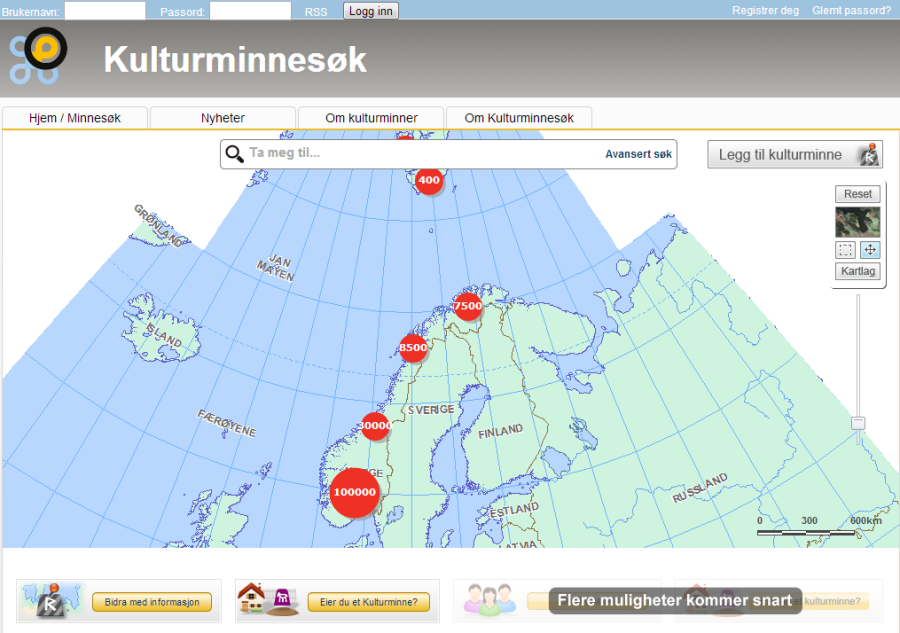
\includegraphics[width=0.8\textwidth]{Figures/Prestudy/kulturminnesokOversikt.png}
      \caption{Kulturminnesøk, Norway}
      \label{fig:pre_kulturoversikt}
\end{figure}

\begin{figure}[H]
      \centering
      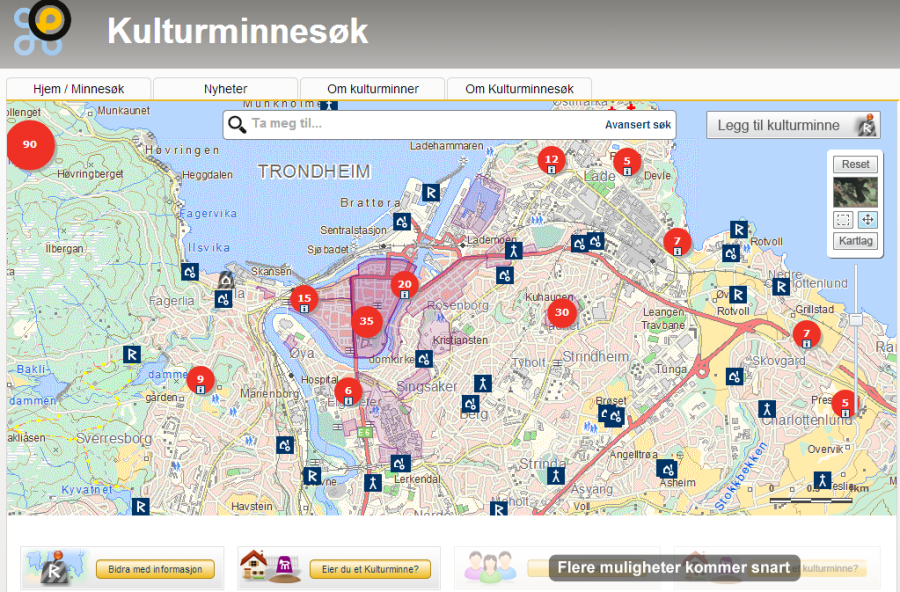
\includegraphics[width=0.8\textwidth]{Figures/Prestudy/kulturminnesokTrondheim.png}
      \caption{Kulturminnesøk, Trondheim}
      \label{fig:pre_kulturTrondheim}
\end{figure}

As you can see in Figure~\ref{fig:pre_kulturoversikt}, sights from all over Norway is represented. We can either press the red circles, zoom in manually or search by text to find places we want to take a closer look at. If we zoom in over Trondheim, as Figure~\ref{fig:pre_kulturTrondheim} shows, there are plenty of sights all over the city. Every sight is marked with a symbol, which tells the user if it is a building location, religious place, archaeological memory or technical/industrial memory. If you click on a symbol, a small info display appears, Figure~\ref{fig:pre_kulturInfo}, that informs the user what type of cultural heritage it is, its conservation status, dating and municipality. If the user wants more info, the user can press the ``Mer info'' (More info)-text, and  a new sight appears, Figure~\ref{fig:pre_kulturMoreInfo}, where a picture, if available, and a some more info appears. It is also possible to comment and like (as in Facebook) the site.

\begin{figure}[H]
      \centering
      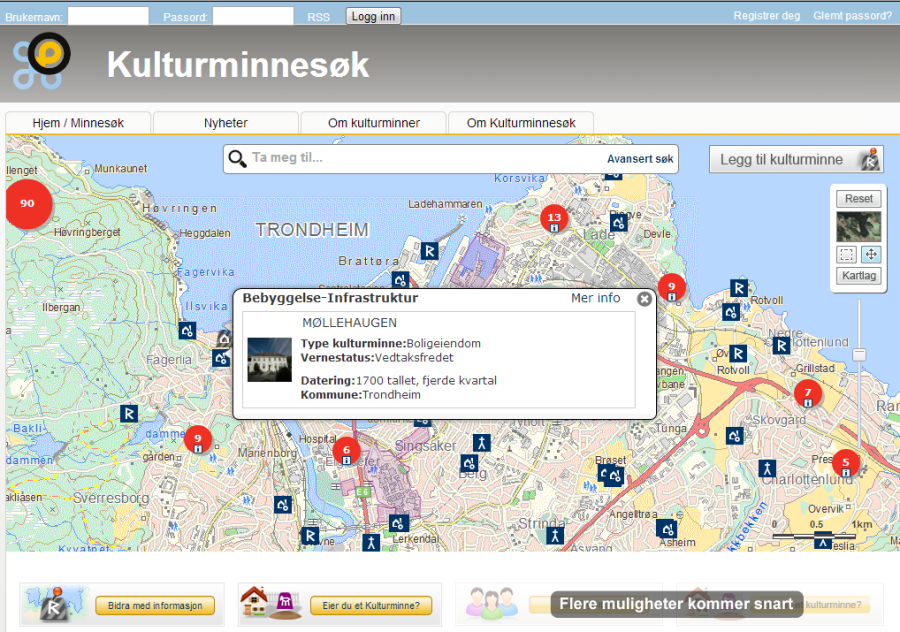
\includegraphics[width=0.8\textwidth]{Figures/Prestudy/kulturminnesokClick.png}
      \caption{Kulturminnesøk, info display}
      \label{fig:pre_kulturInfo}
\end{figure}

\begin{figure}[H]
      \centering
      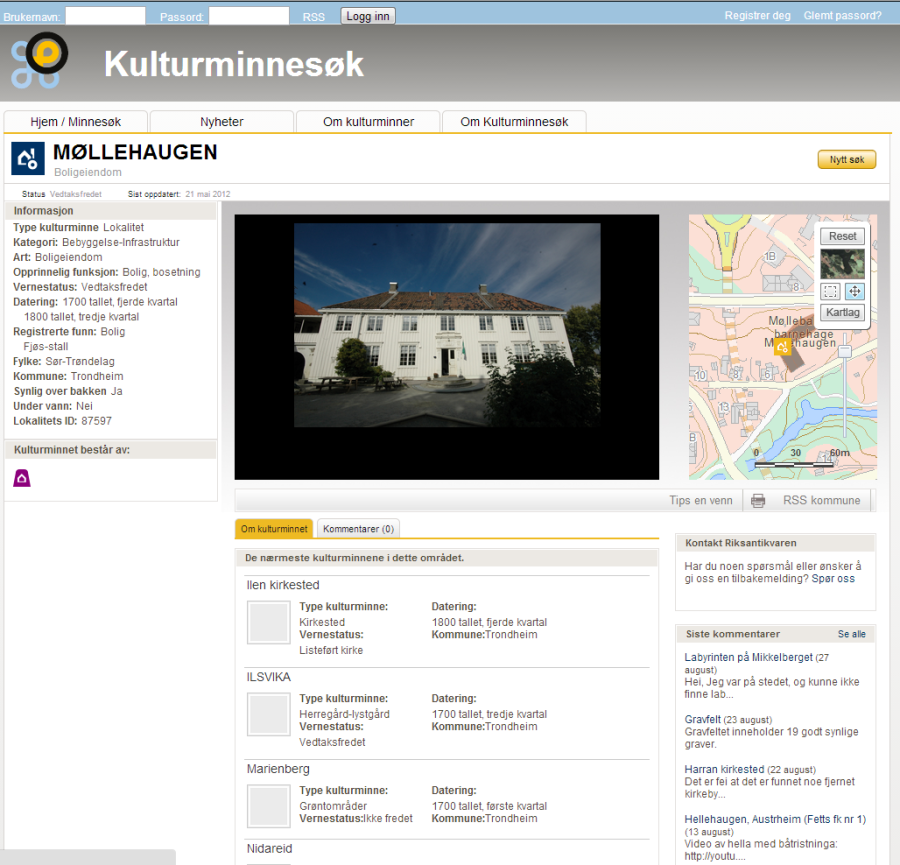
\includegraphics[width=0.8\textwidth]{Figures/Prestudy/kulturminnesokMoreInfo.png}
      \caption{Kulturminnesøk, more info}
      \label{fig:pre_kulturMoreInfo}
\end{figure}

Kulturminnesøk can be considered a partly edge dominant system (will be explained next section), since everyone can register and add their own cultural heritage sight. There is about 1500 sights that users have added. Users have added everything from swimming halls to archaeological memories. We call it just partly edge dominant, since only 1\% of the content is added by the public.

\begin{figure}[H]
      \centering
      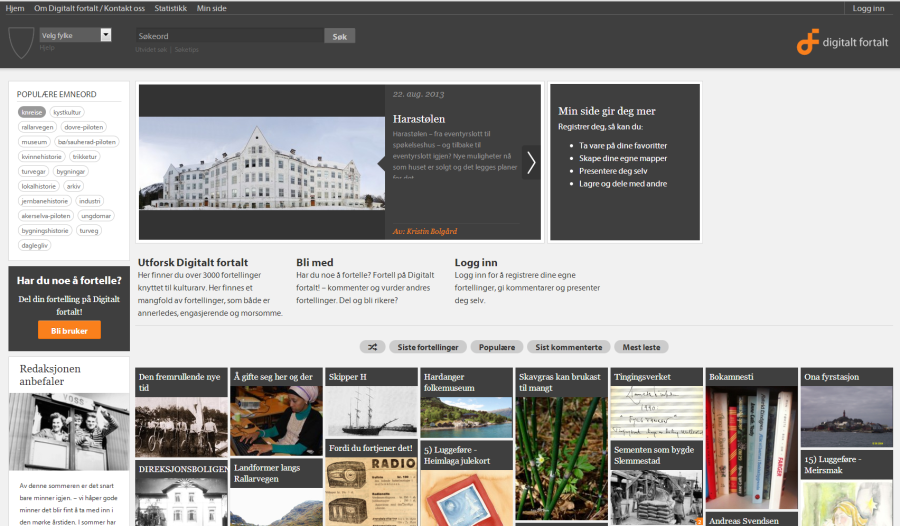
\includegraphics[width=0.8\textwidth]{Figures/Prestudy/digitaltfortaltForside.png}
      \caption{Digitalt fortalt, front page}
      \label{fig:pre_fortaltFrontPage}
\end{figure}

Another edge dominant cultural heritage system is ``digitalt fortalt'', or digitally told. Digitalt fortalt is a website where users, cultural institutions or private persons, can register and add stories related to cultural heritage. Users have added stories about everything from clothespins to protected buildings, and today there are over 3000 stories. 

To read a story you can either search, by pressing one of the popular tags or simply search from the search field, or browse on the front page, in last told stories, popular stories, last commented stories or among the most  read stories. If we search on ``Trondheim'' in the search field, we get 135 hits. The stories is placed in a grid system, and every story is represented in a little box, with a title, a picture (a play-sign if a sound is attached to the story), author and location. Some stories are also linked to a date or a period. The search result is shown in Figure~\ref{fig:pre_fortaltTrondheim}.

If we press one of the stories, Regalierommet for instance, shown in Figure~\ref{fig:pre_fortaltRegalierommet}, a page with a media slider and information appears. In this case the story is represented as sound and pictures. The information below the media slider says something about why it was made, and some information about the creators. In other stories there are typically one or more pictures and the story represented with text.

\begin{figure}[H]
      \centering
      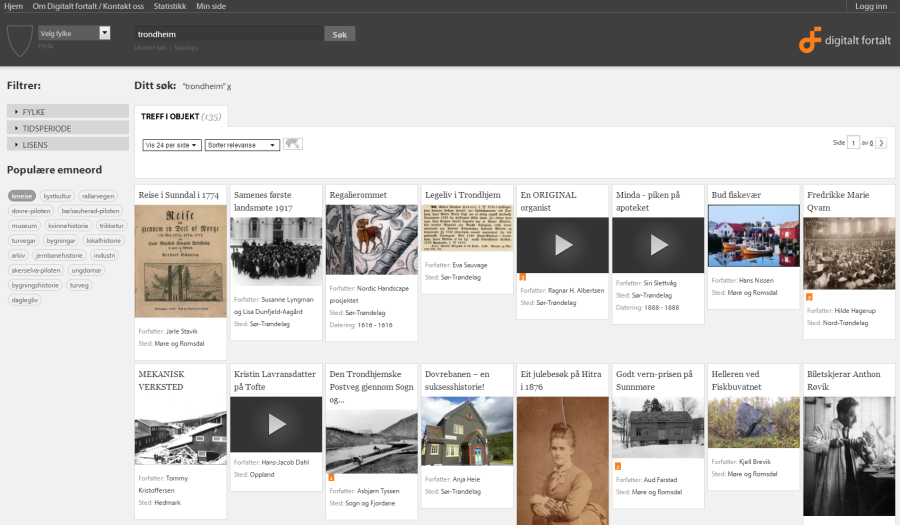
\includegraphics[width=0.8\textwidth]{Figures/Prestudy/digitaltfortaltSokTrondheim.png}
      \caption{ Digitalt fortalt, search result for Trondheim}
      \label{fig:pre_fortaltTrondheim}
\end{figure}

\begin{figure}[H]
      \centering
      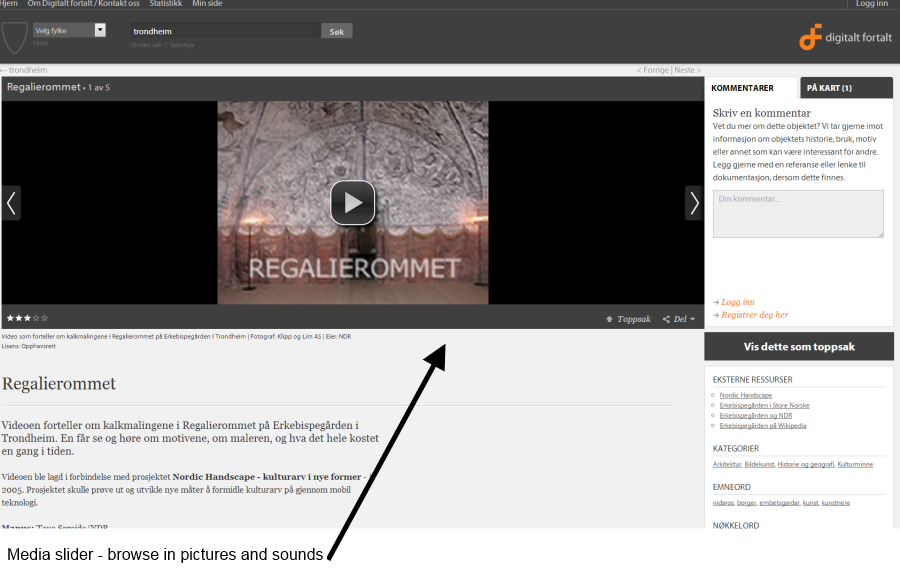
\includegraphics[width=0.8\textwidth]{Figures/Prestudy/digitaltfortaltRegalierommet.png}
      \caption{Digitalt fortalt, Regalierommet, with media slider and text}
      \label{fig:pre_fortaltRegalierommet}
\end{figure}

\subsection{Edge dominant systems}
An edge dominant system is one that almost entirely depends on input from users. Well known edge dominant systems today are Facebook, Twitter, YouTube, Wikipedia, etc., all of which have created enormous value by their users. 

Almost all edge dominant systems today share a common ecosystem structure, called a ``Metropolis'' structure, by analogy with a city, as shown in Figure~\ref{fig:pre_edgeMetropolis}.

\begin{figure}[H]
      \centering
      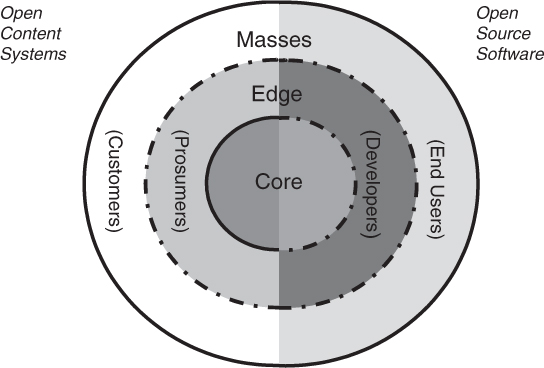
\includegraphics[width=0.8\textwidth]{Figures/Prestudy/metropolis.jpg}
      \caption{The metropolis}
      \label{fig:pre_edgeMetropolis}
\end{figure}

The metropolis structure divides the communities of stakeholders in an edge dominant system:

\begin{itemize}
  \item In the outermost ring we have the masses, consisting of customers and end users. They consume the content made by the metropolis, and contribute requirements.
  \item The middle ring contains prosumers and developers. These are the people that produces the content for the metropolis. The developers write software for the community to use, and the prosumer produce (and consume) content in the metropolis.
  \item In the middle we have the core that keeps the metropolis together. This is the software that provides its services through a set of APIs that the prosumers and developers can use to produce new software and content for the masses to use.
\end{itemize}

\section{Existing mobile applications}\label{sec:prestudy_existing_apps}
In the previous sections we have learned that there already are already systems that helps the public in finding cultural heritage. In this section we will look at some existing mobile applications which in many ways works quite similar to the systems above. It is important to look at these systems to get an idea of how others have done it before us, both to get inspired and to find weaknesses with this kind of applications. First we will take a look at Kulturminnesøk's mobile application, then at two danish solutions.

\subsection{Kulturminnesøk app}
After using Kultruminnesøk in the web browser we discovered that they also had a mobile application. Not surprisingly, it serves much of the same functions as the web application, but has some drawbacks and  advantages. First of all, it has the same map function, Figure~\ref{fig:pre_kulturMinneAppMap}, you can zoom in and out with the well known ``pinch-to-zoom'' gesture, which allows the user to zoom in or out by moving two fingers further apart or closer together while touching the display. The same symbols as in the web application is used, and we can press them to get more information. In addition to the map you can use a list function where you can see your nearest sights, Figure~\ref{fig:pre_kulturMinneAppList}. However, the coolest function is the mobile application is in the function ``Vis meg'', or ``Show me''; this is a augmented reality function, where all sights within a certain range appears on the screen, through a camera application, represented by the same symbols in the map, Figure~\ref{fig:pre_kulturMinneAppAug}.  A quite big drawback is that there are no pictures in the ``More info'' display, but the biggest weakness is that the application does not show user-created sights, just the cultural sights from the Askeladden database.

\begin{figure}[H]
      \centering
      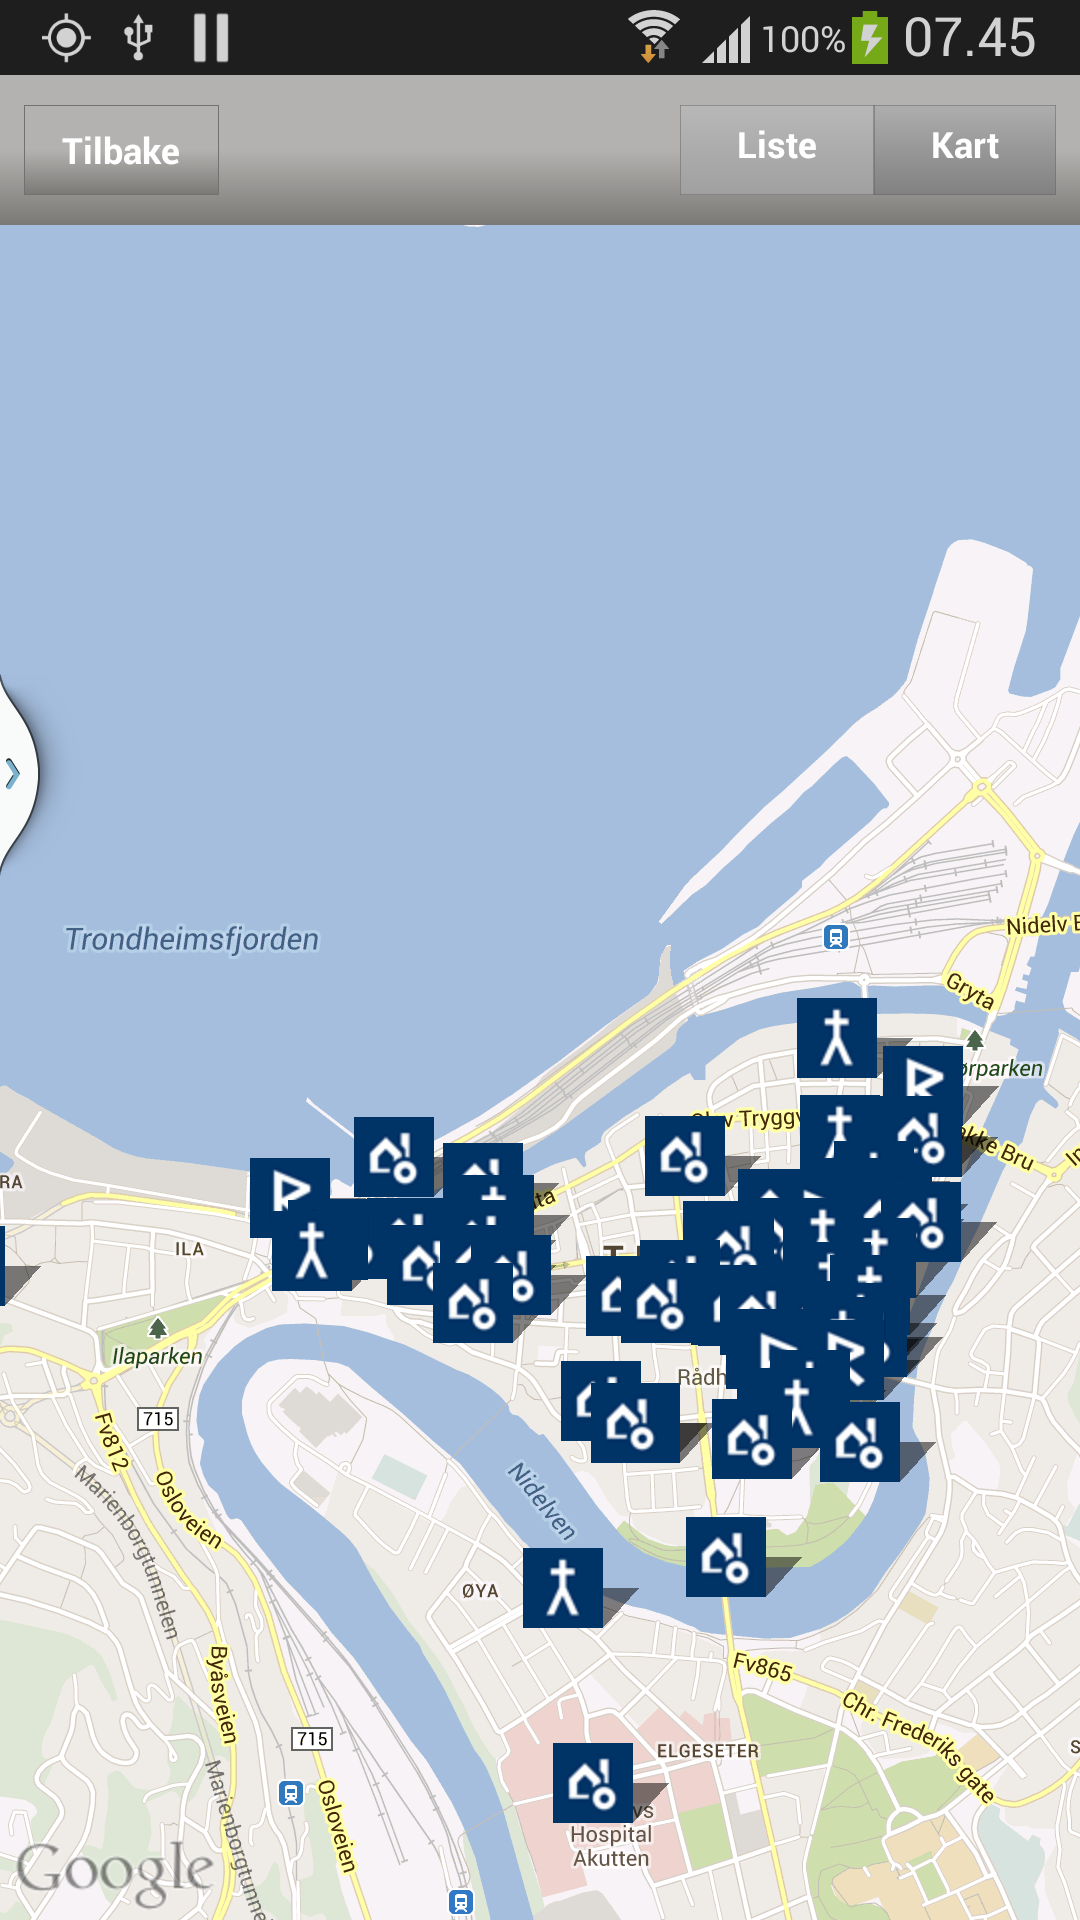
\includegraphics[width=0.4\textwidth]{Figures/Prestudy/kulturSokMap.png}
      \caption{Kulturminnesøk, map function}
      \label{fig:pre_kulturMinneAppMap}
\end{figure}

\begin{figure}[H]
      \centering
      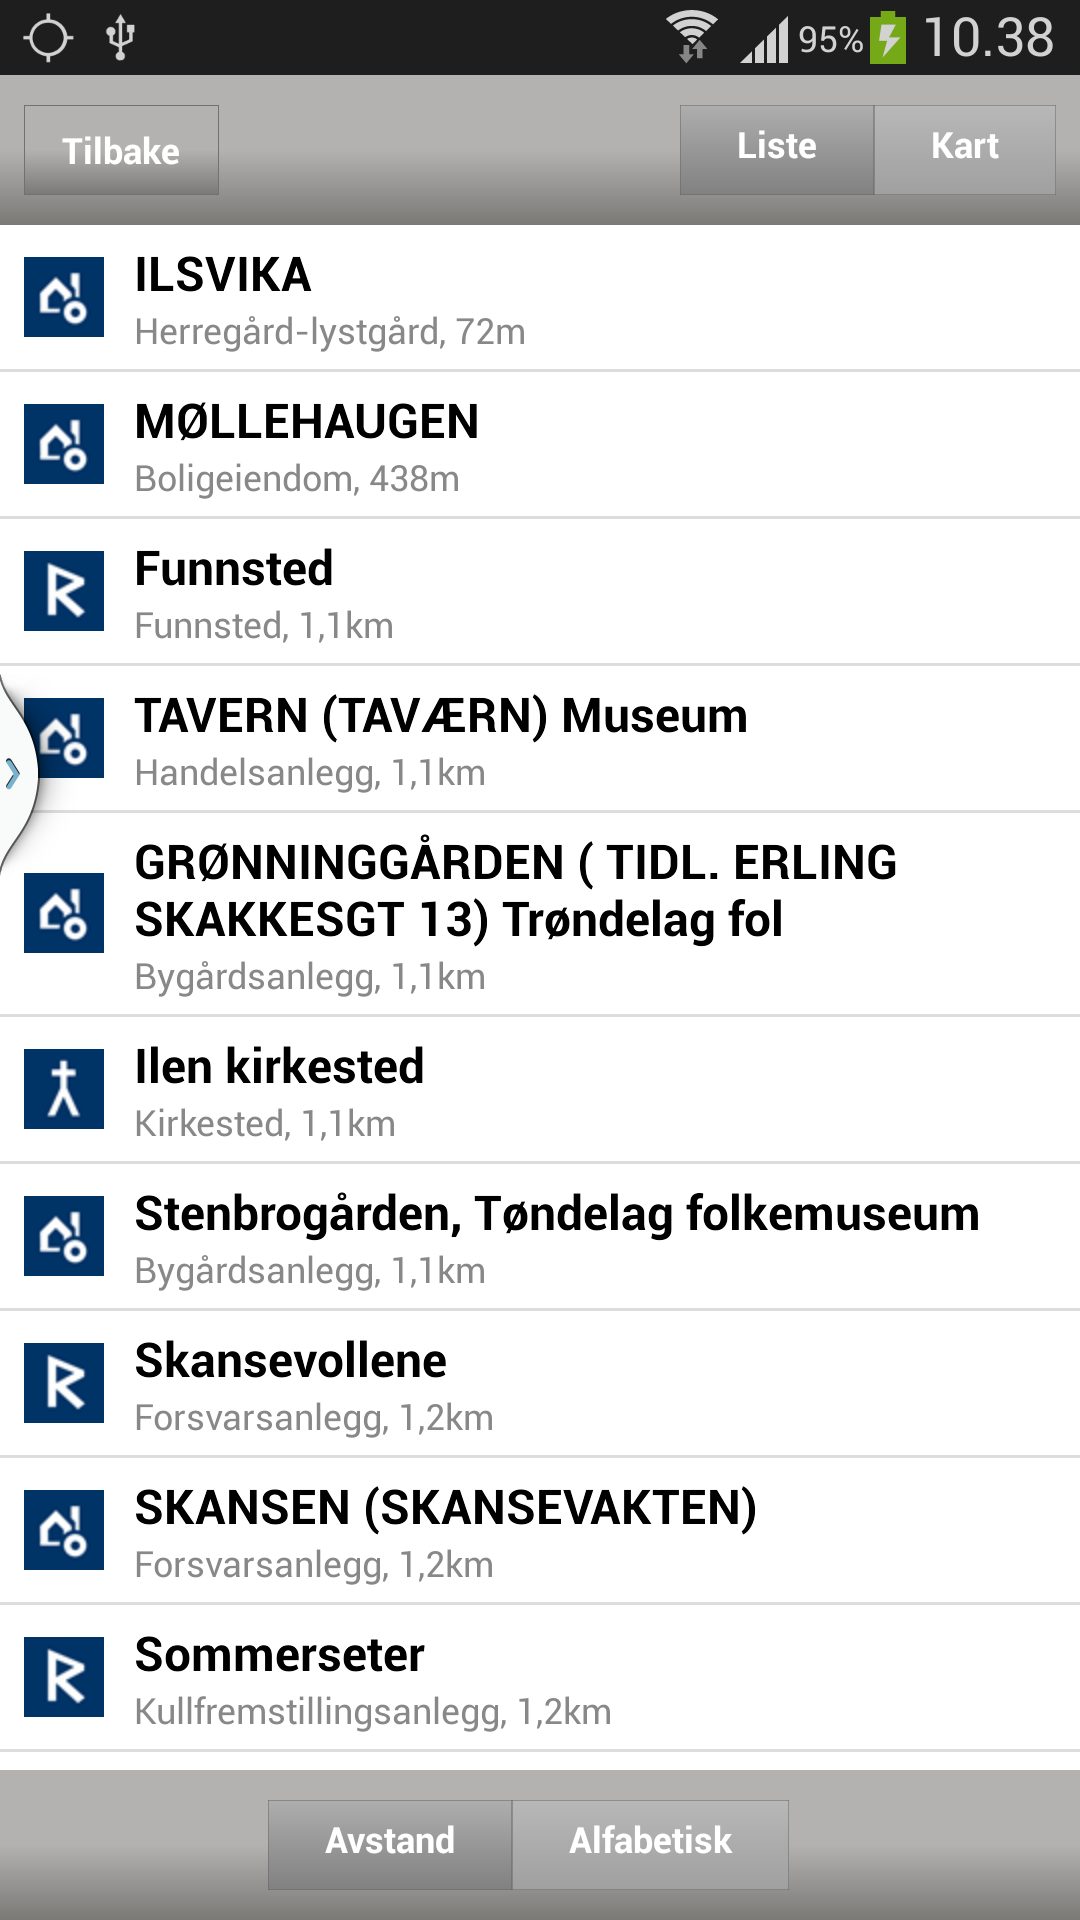
\includegraphics[width=0.4\textwidth]{Figures/Prestudy/kulturSokList.png}
      \caption{Kulturminnesøk, list function}
      \label{fig:pre_kulturMinneAppList}
\end{figure}

\begin{figure}[H]
      \centering
      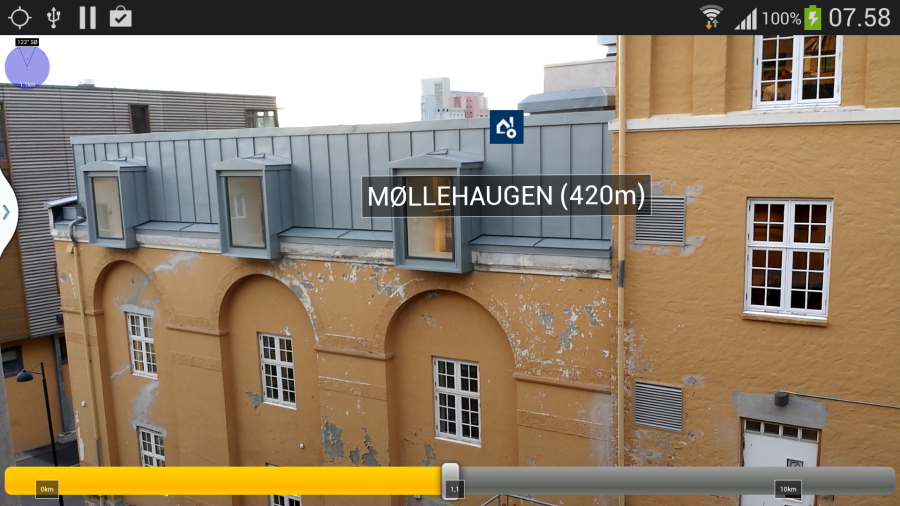
\includegraphics[width=0.8\textwidth]{Figures/Prestudy/kulturSokAR1.png}
      \caption{Kulturminnesøk, augmented reality function}
      \label{fig:pre_kulturMinneAppAug}
\end{figure}

\subsection{Kulturarv app}
Kulturarv, or Cultural Heritage, is a danish cultural heritage mobile application. It is very similar to the Kultursøk mobile application, it has both a map function, Figure~\ref{fig:pre_kulturArvAppMap}, and a augmented reality function, Figure~\ref{fig:pre_kulturArvAppMap},  to show the user where to find protected and preservation-worthy buildings. It uses the danish ``Fredede og Bevaringsværdige Bygninger'', or  ``Protected and Preservation-worthy Buildings'', (FBB) web service, which appears to be quite similar to the Askeladden database. It sounds like the danish Kulturarv and Kultursøk is pretty much the same thing, but Kulturarv has one more important functions, which makes is much better; Kulturarv blends the media from FBB and other geolocation data sources like Instagram, Flickr, Wikipedia and Twitter. Unfortunately, we are not able to test the application because it seems to only work if you are physically in Denmark, but we have the impression of how it works through Kulturarv's homepage \cite{Kulturarv}. It is also worth  mentioning that the application is an open-source project released under the GNU GPL v3 license.

\begin{figure}[H]
      \centering
      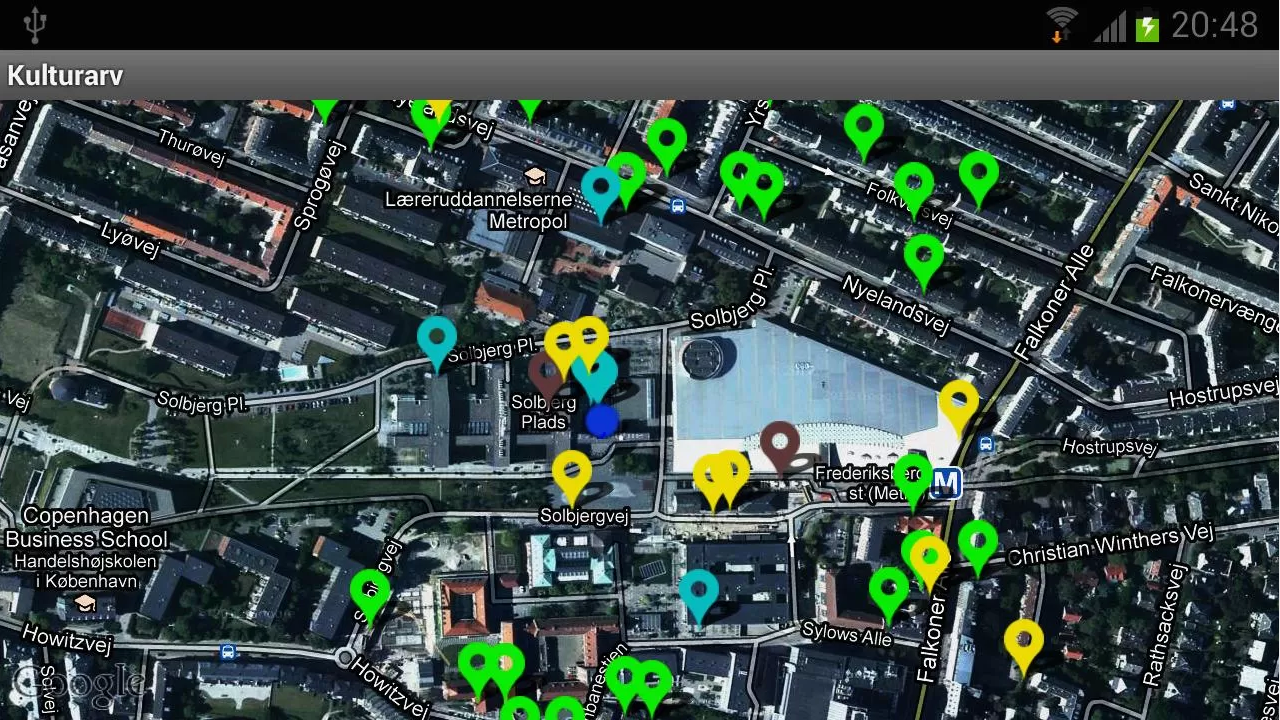
\includegraphics[width=0.8\textwidth]{Figures/Prestudy/kulturArvMap.png}
      \caption{Kulturarv, map function}
      \label{fig:pre_kulturArvAppMap}
\end{figure}

\begin{figure}[H]
      \centering
      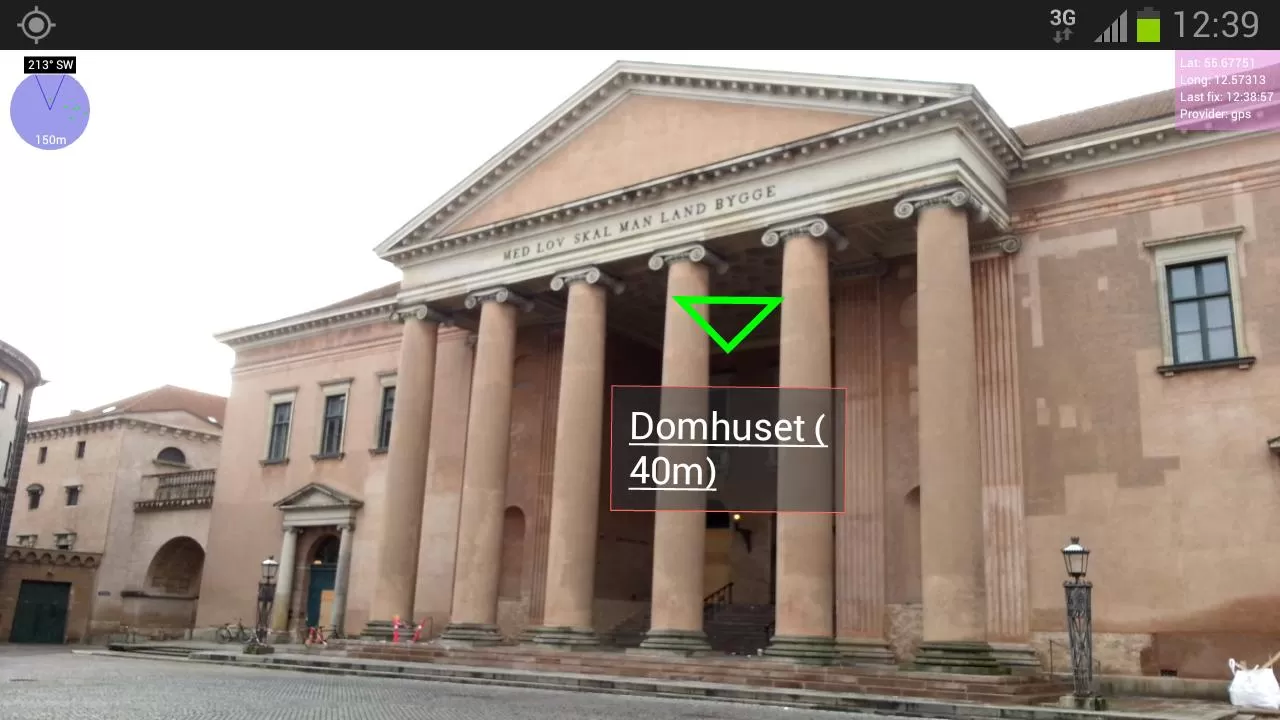
\includegraphics[width=0.8\textwidth]{Figures/Prestudy/kulturArvAR1.png}
      \caption{Kulturarv, augmented reality function}
      \label{fig:pre_kulturArvAppAug}
\end{figure}

\subsection{1001 Stories of Denmark}
Again we are looking at a danish application that has many similarities with a Norwegian application, namely Digitalt Fortalt. It is called ``1001 Stories of Denmark'', and it lets the user read stories about 1001 places in Denmark, including ancient monuments, architectural buildings and sceneries. You can browse sights with either a map or a list, Figure~\ref{fig:pre_1001StoriesDenmarkAppList} and~\ref{fig:pre_1001StoriesDenmarkAppMap}. When you choose a sight, you can read about the sight in general, read stories about it or look at pictures, Figure~\ref{fig:pre_1001StoriesDenmarkAppStory}. Another function is that you can get predefined routes or make your own routes, that includes the sights you want to see. For example, you can find a route that is about the famous architect and designer Arne Jacobsen (1902 - 1971), that includes visits to buildings that was designed by Arne Jacobsen. In the same way as the previous application, we can not test it because you need to physically be in Denmark.

\begin{figure}[H]
      \centering
      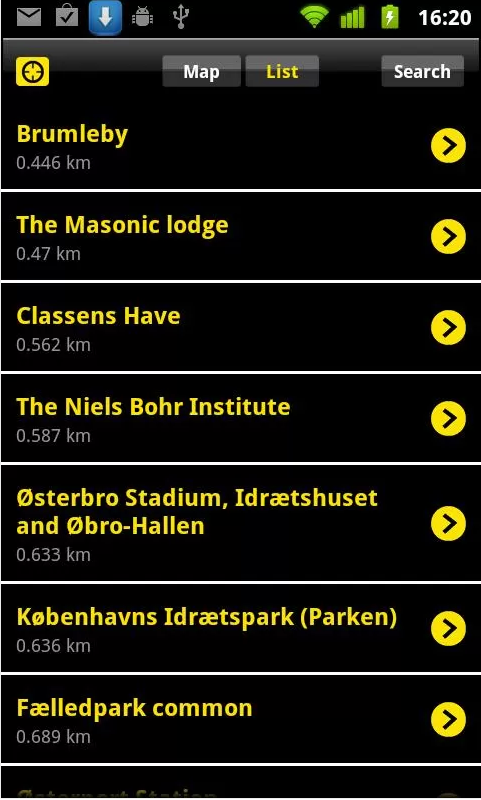
\includegraphics[width=0.3\textwidth]{Figures/Prestudy/1001storiesList.png}
      \caption{1001 Stories of Denmark, list function}
      \label{fig:pre_1001StoriesDenmarkAppList}
\end{figure}

\begin{figure}[H]
      \centering
      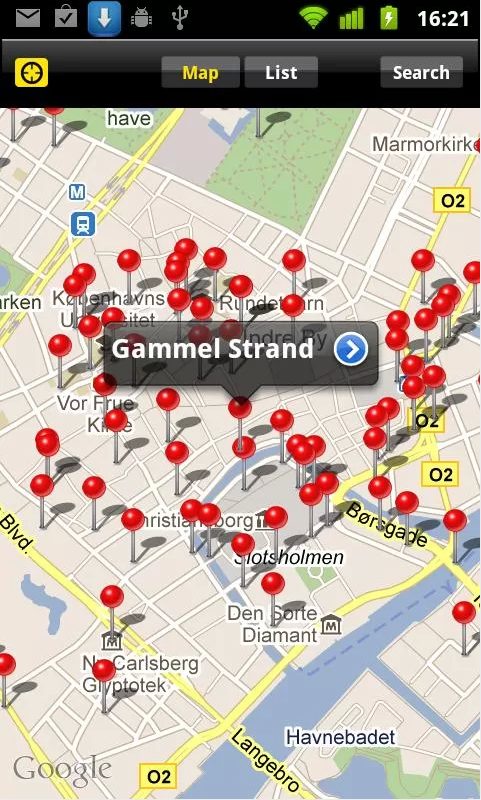
\includegraphics[width=0.4\textwidth]{Figures/Prestudy/1001storiesMap.png}
      \caption{1001 Stories of Denmark, map function}
      \label{fig:pre_1001StoriesDenmarkAppMap}
\end{figure}

\begin{figure}[H]
      \centering
      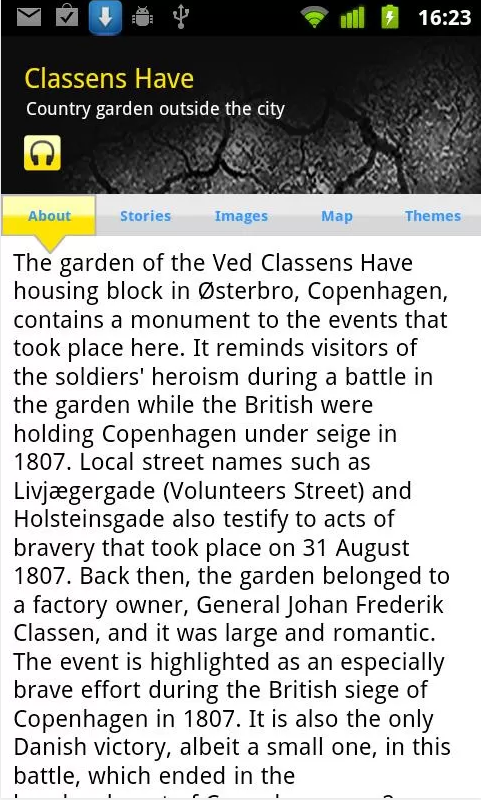
\includegraphics[width=0.4\textwidth]{Figures/Prestudy/1001storiesStory.png}
      \caption{1001 Stories of Denmark, a sight}
      \label{fig:pre_1001StoriesDenmarkAppStory}
\end{figure}

This mobile application also has an associated website \cite{1001fort}, where you have the same functions as in the mobile application. In addition there is a timeline function, where all the stories with a timestamp appears, Figure~\ref{fig:pre_1001StoriesDenmarkTimeLine}. The website also invites users to create their own profile, that allows them to add and recommend places, add stories, comment on existing stories and to  upload images and videos.

\begin{figure}[H]
      \centering
      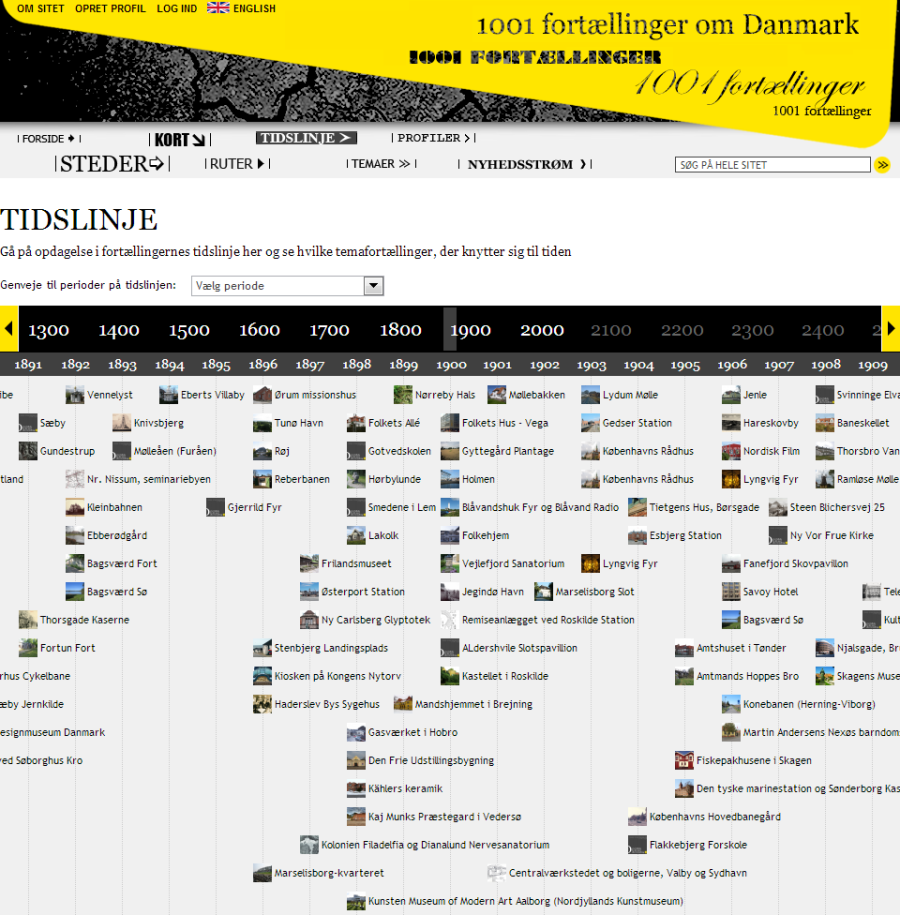
\includegraphics[width=0.8\textwidth]{Figures/Prestudy/1001storiesWebsiteTimeline.png}
      \caption{1001 Stories of Denmark,timeline function}
      \label{fig:pre_1001StoriesDenmarkTimeLine}
\end{figure}

\subsection{Conclusion}
All the applications we have looked at are great pieces of technology. It educates today's generation and helps them discover and learn about our cultural heritage. They are all content-rich applications, and they offers the public to contribute. One thing we have noticed is that nearly every sight, story, place or piece of history are pretty thoroughly made. Perhaps we should focus on a more low-threshold application, so that everyone, even the very young, can participate.
We see that every applications has their own advantages, and we hope that we can purify some of these and perhaps even come up with some new revolutionary features.


\section{Work methodology}
There are different ways of approaching a project. Two of the more commonly used methods is Waterfall and SCRUM.

\subsection{Waterfall}
The Waterfall model \cite[p. 30-32]{Sommerville10} is derived from general system engineering processes.The work done in a Waterfall model is partitioned in activities. The activities are done sequentially, only when the prior is done, can the consecutive start.

\begin{figure}[H]
      \centering
      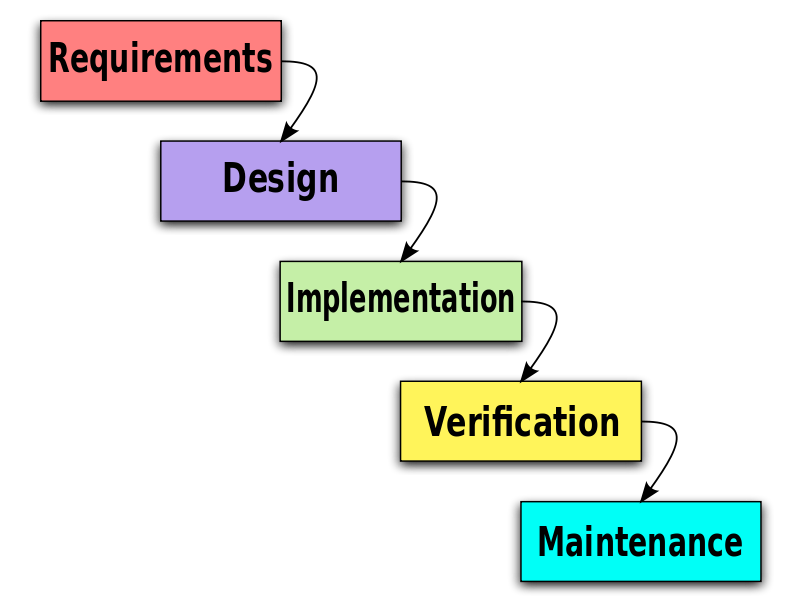
\includegraphics[width=0.8\textwidth]{Figures/Prestudy/Waterfall.png}
      \caption{The Waterfall process \cite{wikipedia:waterfall}}
      \label{fig:pre_waterfall}
\end{figure}

Every phase produces one or several documents to be passed on to the next phase. These documents needs approval before a phase is considered completed, and the next might start.

Waterfall makes good sense in larger manufacturing environments where certification of every part of the system is required in order to be allowed to manufacture and sell the product. For example the aircraft industry needs detailed plans of the whole aircraft to be certified before manufacturing, and faults could produce devastating effects.

In the original publication about Waterfall for software systems, the author raises some limitations of the model and suggests some project owner involvement.

\begin{quotation}
For some reason what a software design is going to do is subject to wide interpretation even after previous agreement. It is important to involve the customer in a formal way so that he has committed himself at earlier points before final delivery. To give the contractor free rein between requirement definition and operation is inviting trouble. \cite[p. 335]{DBLP:conf/icse/Royce87}
\end{quotation}

\subsection{SCRUM}
In accordance with the statement from Royce above, SCRUM strive to involve the customer throughout the whole development process. This is done by doing only the strictly required planning and specification writing up front, and then working iteratively with the project together with the customer in sprints. According to \cite[p. 73]{Sommerville10} sprint could last from 2 - 4 weeks and by the end the work is review and result presented for the customer. For each sprint the customer sees the current state of the project and participates in specifying what to do for the next sprint.

\begin{figure}[H]
      \centering
      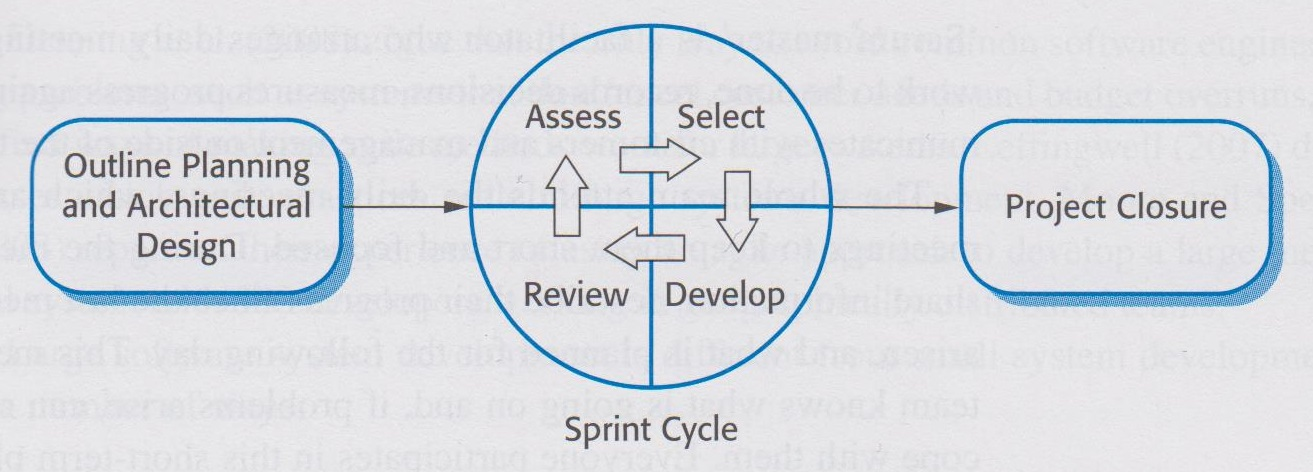
\includegraphics[width=0.8\textwidth]{Figures/Prestudy/SCRUM.jpeg}
      \caption{The SCRUM process}
      \label{fig:pre_scrum}
\end{figure}

This use of continuous customer involvement, helps clarifying misunderstandings and correcting errors on both the customers and contractors side during the process. The fact that this might be caught earlier, means that the project is more likely to deliver on time and on budget.

The customer involvement is primarily within prioritizing and adding items to the backlog which is used as the basis for each sprint. The customer is also involved in clarifying items as they are moved from the backlog to the sprint log.


\subsection{Chosen work methodology}
Given the uncertainties surrounding the concrete goal and plan behind the project, it is beneficial to choose SCRUM to retain a close connection with the customer. This will help resolve any misunderstandings or disagreements about project scope and focus areas.

The customer have experience with SCRUM and suggested the methodology to be used. It will also make it easier to produce a good end project, knowing that we are allowed to refine our documents, requirements and such during the lifetime of the project.

\chapter{Requirements} \label{chap:req}

This chapter is a System Requirements Specification document in the terms of practice recommended by IEEE 830 \cite{ieee830}.

\section{Introduction}

\subsection{Purpose}
The purpose of this document (System Requirements Specification, hereinafter SRS) is to collect and analyze the requirements for VirtualWall software system. The requirements formalization as presented is a result of a joint effort of the customer and the development team. It serves as a description of what customer is expecting the system to be like, it presents the systems features and functionalities.

The intended audience of this document shall be:

\begin{enumerate}
  \item development team (students)
  \item customer (SINTEF ICT, eTrøndelag/Sør-Trøndelag fylkeskommune)
  \item course responsibles (advisor, etc.)
\end{enumerate}

Each part of the audience holds different stakes in the project, but all are interested in information contained within the SRS.

\subsection{Scope}
This SRS document deals with the project Virtual walls – walls that tell us stories. This project shall result in developing a tool for working with so called virtual walls, creating and sharing stories on them.

As presented by customer, the VirtualWall software system is going to be a complex system consisting of a number of subsystems including several content databases, a server backend and web application frontend.

In the scope of this year's run of Customer Driven Project course, a prototype of a web application frontend and a basic server backend shall be developed.

\subsection{Definitions, acronyms and abbreviations}

\begin{table}[H]
\centering
\begin{tabular}{ l  p{11cm} }
	AJAX 			& Asynchronous JavaScript and XML 																					\\ \hline
	HTML 			& HyperText Markup Language 																						\\ \hline
	HTTP 			& HyperText Transfer Protocol 																						\\ \hline
	JSON 			& JavaScript Object Notation 																						\\ \hline
	Virtual Wall 	& By virtual wall, we understand a virtual space where users can share stories like on a real-life wall. 
						Stories can be textual, as well as featuring interactive media like video, audio, images or hypertext. 			\\ \hline
	Owner 			& All items (walls, stories) in the system are created by someone. We call this user owner of the underlying entity \\
\end{tabular}
\label{tab:req_definitions}
\caption{Definitions, acronyms and abbreviations}
\end{table}

\subsection{Overview}
The rest of this SRS document describes the proposed product in the means of its desired functionality, characteristics, constraints and perspectives. This general description could be found \ref{sec:req_overall_description}. Description of the actual requirements is to be found in \ref{sec:req_specific_requirements}.

\section{Overall description}\label{sec:req_overall_description}
\subsection{Product perspective}
As stated above, the whole system will consist of several subsystems such as the frontend, server backend, own database and external content databases. This implies the use of client-server model.

The components developed in this phase of the project are:

\begin{enumerate}
  \item mobile/web application (frontend)
  \item server (backend)
\end{enumerate}

Customer requires that the tool shall be available for PCs, tablets and mobile phones (smartphones). The prototype shall be optimized for a tablet preferably.

The following diagram shows the whole system and how the separate parts work together.

\begin{figure}[H]
      \centering
      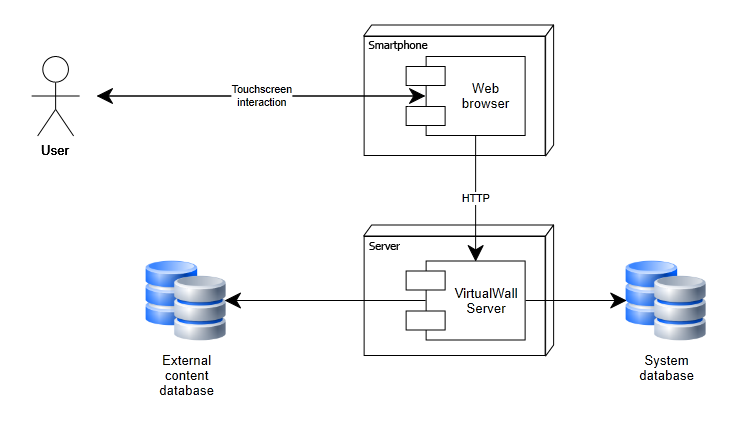
\includegraphics[width=0.8\textwidth]{Figures/Requirements/overview.png}
      \caption{Overview of interaction}
      \label{fig:req_overview}
\end{figure}

In the initial phase, the server will not be directly connectex to any external content databases machine, the content from them would be presented as simple hyperlinks leading to the third party website (such as kulturminnesok.no, digitaltfortalt.no).

\subsection{User Interfaces}
Since the frontend of the whole system shall be developed in this project, the description of user interface shall be considerably stressed.

We can characterize the nature of the system as crowdsourced (or edge-dominant, in general), as the content shall be generated and modified by users to some extent. Due to this, there is not going to be any backend for data entry, the only point where the system is exposed to human beings is the web application frontend.

Our key quality attribute, usability, relates tightly to user interfaces. For this reason, all usability-related requirements on user interface are listed in section \ref{sec:req_software_system_attributes} as quality attribute requirements.

\subsubsection{Web application front end}\label{sec:req_webapplication_frontend}
As user requests that the initial prototype application shall be developed for use on tablets. Typical usage of the system suggests that it will be used in field, which implies using the application on smartphones and tablets.

Both smartphones and tablet have some inherent characteristics that have to be respected when designing the user interface and the means of interacting with it.

The screen sizes of current smartphones vary a lot, with the most phones with screen size from 3.5 inches (9 cm) up to 5.5 inches (14 cm). Screen sizes of tablets vary between values from 9 inches (22 cm) to 11.5 inches (29 cm). In addition, these devices can be used in either landscape or portrait mode.

Such a diversity in screen sizes makes designing the user interface very challenging. On one hand, we want to maximize the screen usage even on large-screen devices, on the other hand, we must make the application usable even on devices with screen area up to 9 times smaller.

Another characteristic property of those devices is that their interaction mechanisms are somewhat limited.

\begin{enumerate}
  \item These devices are generally missing a mouse, and thus a mouse cursor. Direct pointing is done by using finger upon touchscreen. This is however less precise, so the user interface must be accustomed to that.
  \item Devices usually miss a hardware keyboard. This is surrogated by having a software keyboard on-screen. This however takes up some of the valuable screen real estate. This kind of keyboard is additionally not as usable as a real hardware one, so the user is not tempted to use it as much., therefore use of any hotkeys is out of question.
\end{enumerate}

\subsection{Software interfaces}
We imply that the server and the client interoperate and are developed to work with one another. The required interfaces and communication schema is to be determined later on.

\subsection{Communication interfaces}
Another inherent characteristic of mobile devices (smartphones, tablets, etc.) is the unreliability and speed of network connection. Since this application is a part of a client-server system, the communication link between those is critical.

The main issues with mobile data networks are frequent interruption, big latency and small bitrate. Sometimes the connection can as well be unavailable at all. This results in the data connection being slow and unreliable which has a great significance on the performance of the application and its usability. As developers of the web application, we need to take this into consideration.

There are several techniques how to deal with mentioned issues or at least mitigate their impact.

\subsubsection{Unavailability of connection}\label{sec:req_unavailability_of_connection}
To deal with frequent interruption and unavailability of connection, an off-line mode of the application could be implemented in the future, which would enable the user to work without a network connection (in a limited way).

This was described by the customer as to be a low priority requirement, not to be implemented in this phase.

\subsubsection{Small throughput}
To deal with small throughput of the network, the updates of the content in the client application could be implemented using delta updating. This would mean only new and changed data are sent from the server, data that did not change are used from the local storage.

This issue is not to be addressed in this phase of the project and may be implemented later on.

\subsection{Product functions}

\subsubsection{Frontend}
The key functionality expected in the frontend is management of virtual walls (creating, editing), stories on them (creating, editing) and social interaction (commenting, sharing).

\subsubsection{Backend}
The key functionality of the server is to support the features of the client by storing the data in the database and retrieving it back. As said above, the content is stored in the system database. The server shall expose an API for accessing the items from database (walls, stories) for access from the frontend.

\subsection{User characteristics} \label{sec:req_user_characteristics}
As this app shall be accessible to open public, we can neither anticipate users' educational level, nor experience, nor technical expertise. We can however assume basic computer literacy.

Documentation from customer features a scenario how this application would be used in class in elementary school. We may anticipate that some of the users can be as young as 10 years for example.

See chapter \ref{sec:req_usability} for requirements on usability.

\subsection{Constraints}

\subsubsection{HTML5 use}
Since use on many different devices and platforms is expected and necessary, customer requested that the frontend would be a web application. As the system is crowdsourced and heavily relies on users, it it necessary that it interacts very well with the users and is visually appealing. Also, for reasons stated in \ref{sec:req_unavailability_of_connection}, local storage is necessary to enable off-line mode (in the future). This implies the use of cutting-edge technologies for the development.

For this reason, customer suggests that the application will be developed in HTML5.

\section{Specific requirements}\label{sec:req_specific_requirements}

\subsection{External interfaces}
As the application developed is going to be a client/server where the client is a web application, we will use HTTP protocol for data exchange. Data transferred over HTTP in our case will be in HTML and XML or JSON formats. This is to be determined later.

\subsubsection{Virtual Wall Client/Server interface}
VirtualWall client is a classic web application that runs in a web browser. This implies that is will be downloaded via HTTP as a HTML document.

Once the web application is open in the browser, data transfers with the web server can be done using AJAX to retrieve the data in XML/JSON format from the server.

Format of the messages shall be determined later.

\subsubsection{Social networks}\label{sec:req_social_networks}
Walls and stories shall be easily shared using social networks like Facebook or Twitter. Custom button for sharing/liking shall be available for each story or wall that user wants to like or share.

Sharing in this case means posting a link on user's social network profile.

\subsection{Functions}
The functional requirements are organized according to object categories.

\subsubsection{Users}

\begin{table}[H]
\centering
\begin{tabular}{ l  p{11cm} }
F1 & System shall let users to register an account within the system\\
\end{tabular}
\label{tab:req_users}
\caption{Users}
\end{table}

\subsubsection{Walls}

\begin{table}[H]
\centering
\begin{tabular}{ l  p{11cm} }
	F2.1 	& System shall enable management of virtual walls 																	\\ \hline
	F2.1.1 	& System shall let registered users create a virtual wall 															\\ \hline
	F2.1.2 	& System shall let owner delete a virtual wall 																		\\ \hline
	F2.1.3 	& System shall enable owner to add contributors to wall (their stories for this location shall appear on the wall) 	\\ \hline
	F2.2 	& System shall let users filter and view walls 																		\\ \hline
	F2.2.1 	& System shall let users to filter walls by popularity 																\\ \hline
	F2.2.2 	& System shall let users to filter walls by tags 																	\\ \hline
	F2.2.3 	& System shall let users to filter walls by metadata (wall owner, location) 										\\ \hline
	F2.2.4 	& System shall let users to filter walls by story authors 															\\ \hline
	F2.2.5 	& System shall show user a list of walls that feature his stories 													\\ \hline
	F2.3 	& System shall let registered users comment on walls 																\\ \hline
	F2.4 	& System shall let users like and share wall over social networks (facebook, twitter).
				See \ref{sec:req_social_networks} for details 																	\\ 
\end{tabular}
\label{tab:req_walls}
\caption{Walls}
\end{table}

\subsubsection{Stories}

\begin{table}[H]
\centering
\begin{tabular}{ l  p{11cm} }
	F3.1 	& System shall enable management of stories on virtual walls 														\\ \hline
	F3.1.1 	& System shall let registered users add story to a location 														\\ \hline
	F3.1.2 	& System shall enable the stories to contain text, hyperlinks, video, pictures, audio 								\\ \hline
	F3.2 	& System shall let users filter and view stories from a particular wall 											\\ \hline
	F3.2.1 	& System shall let users to filter stories by popularity on a particular wall 										\\ \hline
	F3.2.2 	& System shall let users to filter stories by tags on a particular wall 											\\ \hline
	F3.2.4 	& System shall let users to filter stories by metadata (author, media duration) on a particular wall 				\\ \hline
	F3.3 	& System shall let users comment on stories 																		\\ \hline
	F3.3.1 	& System shall notify story author about new comment 																\\ \hline
	F3.3.2 	& System shall enable users to flag a comment as a spam 															\\ \hline
	F3.3.3 	& System shall notify story author about spam-flagged comment 														\\ \hline
	F3.3.4 	& System shall enable story author to remove a comment 																\\ \hline
	F3.4 	& System shall let users like and share stories over social networks (facebook, twitter). 
				See \ref{sec:req_social_networks} for details 																	\\ \hline
	F3.5 	& System shall show user a list all his stories, and for each story a list of walls featuring the story 			\\ \hline
	F3.6 	& System shall notify the user when last wall featuring his story was removed
	\end{tabular}
\label{tab:req_stories}
\caption{Users}
\end{table}

\subsection{Software system attributes}\label{sec:req_software_system_attributes}
In this section, we describe several quality attributes this system shall have.

\subsubsection{Maintainability}
Customer stated that the system shall be well documented and easily extensible and modifiable. These concerns are related to the quality attribute of maintainability.

Customer requests that the project documentation shall include description of all interfaces, architectural description and sequence diagrams to illustrate how does the system work.

\subsubsection{Portability}
As customer requested, the front end application shall be developed in order to be working on various devices, ranging from small smartphones to desktop stations.

Quality attribute scenario to evaluate the system shall be determined later.

\subsubsection{Usability}\label{sec:req_usability}
From the description of typical usage (mentioned in \ref{sec:req_user_characteristics}) and characteristic problems listed in \ref{sec:req_webapplication_frontend}, we came up with several usability scenarios that shall evaluate the usability quality of the software system. As usability is a big concern in this project, usability scenarios and tests shall be included in the report under Test Procedures Specification.  % FIXME SIMON: once usabilitz tests are prepared, put refs to them (link to Test Procedures Specification)

These scenarios shall evaluate, whether the application suits the needs of the audience in the means of usability. These shall be derived from use cases and requirements.

\section{Use case diagrams}
Same categorization as in Functions. 

\subsubsection{User registration}
\begin{figure}[H]
      \centering
      
\includegraphics[width=0.8\textwidth]{Figures/Requirements/user_registration.pdf}
      \caption{Use case diagram for Users}
      \label{fig:req_usecase_users}
\end{figure}

\subsubsection{Walls}
\begin{figure}[H]
      \centering
      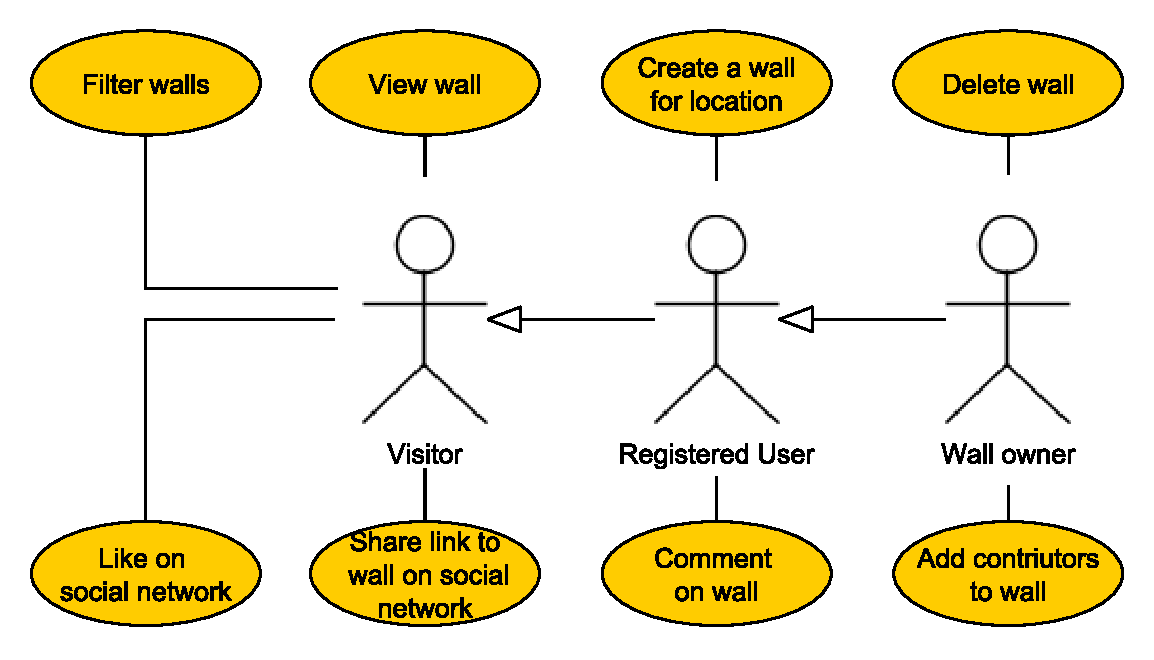
\includegraphics[width=0.8\textwidth]{Figures/Requirements/wall.pdf}
      \caption{Use case diagram for Walls}
      \label{fig:req_usecase_walls}
\end{figure}

\subsubsection{Stories}
\begin{figure}[H]
      \centering
      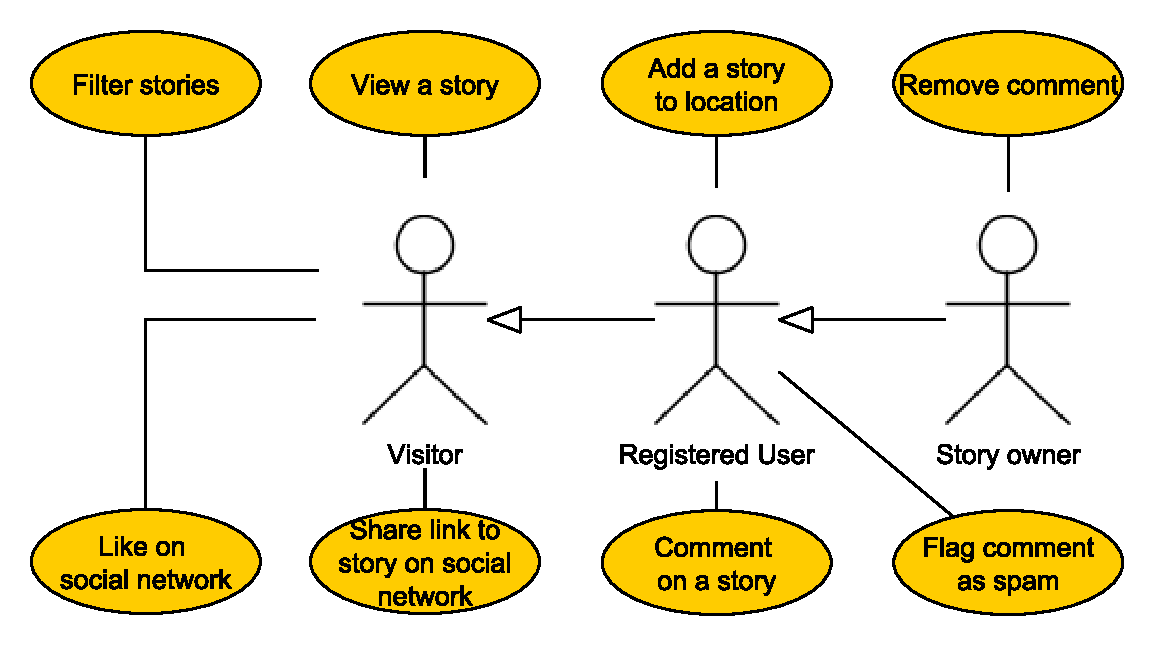
\includegraphics[width=0.8\textwidth]{Figures/Requirements/story.pdf}
      \caption{Use case diagram for Stories}
      \label{fig:req_usecase_stories}
\end{figure}


\chapter{Architecture}\label{chap:architecture}

\section{Architectural drivers} \label{sec:architecture_drivers}
In the following the document, the following items have been used as the main drivers for the architecture.

\subsection{Maintainability} 
A maintainable code base makes for a developable code base. Achieving a maintainable base will make development easier in the short run and maintenance less expensive in the long run. It will also be easier for other teams to continue the development upon the same code base.\\
Quality requirement: Modifiability

\subsection{Portability}
The customer requested that the system should be usable on different smartphone platforms and also on a normal computer. As such portability is key in order to lighten the workload required to achieve this goal.\\
Quality requirement: Modifiability

\subsection{Division between logic and presentation}
Division between logic and presentation makes the system more modular and modifiable.\\
Quality requirement: Usability, Modifiability

\subsection{Short development time}
Given the relatively short duration of this project, the architecture should make for fast development, while not sacrificing quality.

\section{Stakeholders and concerns}

\subsection{Developers}
The architects and developers are concerned about ease and speed of development. As part of this also comes the elegance of the resulting architecture with those in mind that are to continue the development or maintain an operational system.

\subsection{Customer}
The customer is interested in seeing a highly usable system that can run on multiple different devices and be easy to build upon, should they decide to use the prototype as starting point for an actual product.

\subsection{End users}
End users are mostly concerned about the ease of use of the system. This includes the stability and performance as well as the normal usability.

\subsection{Course staff}
The course staff is mostly concerned about the quality of the documentation and its readability.

\section{Selection of Architectural views}
``The 4+1 View Model of Software Architecture'' \cite{Kruchten:1995:VMA:624610.625529} outlines several ways of presenting different aspects of the architecture, useful to different persons. The article uses a variant of Booch syntax to visualize the views, but in this document we will use standard UML diagrams.

This description will focus on the first three views, logical, process and development view.

\subsection{Logical view}
Purpose: The logical view will give us an understanding of how to layout our code in a meaningful way. It will show how classes and modules relates to each other, and as such help us identify common relations and tasks and then generalize them.\\
Stakeholders: Developers, course staff\\
Form of description: Class diagram

\subsection{Process view}
Purpose: The process view serves to show how the modules and classes communicates with each other, and explain the system processes.\\
Stakeholders: Developers, Customer, End users, Course staff\\
Form of description: 

\subsection{Development view}
Purpose: The main matter of concern for the development view is the development process. It serves to show which parts of the system depends upon others. \\
Stakeholders: Developers\\
Form of description: Architecture Layer Diagram

\section{Architectural Tactics}

\subsection{Modifiability}

\subsubsection{Increase cohesion}
By making every part of the system do only one thing, but do it well, it will be easier to change parts of the system or reuse it in other parts.

\subsubsection{Decrease coupling}
By reducing the coupling the change or modification of parts of the systems will have less impact on the rest of the system. Thus making modifications easier.

\subsubsection{Information hiding}
Information hiding allows to provide a stable internal API. This will reduce development time, increase testability and also provide better modifiability.

\subsection{Usability}

\subsubsection{User initiative}
By allowing the user to abort operations, undo or redo the user will feel more comfortable and secure while using the application.

\subsubsection{User model}
By storing the users credentials, the user will not have to provide the credentials every time he executes an action, like requesting content.

\subsection{Testability}

\subsubsection{Limit complexity}
By doing what can be done simple, in a simple way, the system will be less complicated to test and more likely than not have less bugs.

\subsubsection{Local state}
By keeping the state local, the complexity of state machines with multiple participants are avoided. Make central access point stateless, and keep track of the state on the local devices.

\section{Architecture and design patterns}

The overall architecture for the whole system is client-server, where the handheld device or the web browser requests information from the server, which in turn returns it. The advantage of using client-server is that multiple devices might access the same information without needing to download an entire library every time someone updates some information. Using client-server instead of peer-to-peer simplifies keeping the integrity of the information and securing the users data.

\subsection{Client}
On the client Model View Controller will be used in order to separate concerns and keep the code as clean as possible. By dividing user interface, data and logic in different blocks, we increase modifiability and maintainability as well as increasing the speed of development as subdividing tasks will be easier.

The client might even be Model View Presenter (MVP). This uncertainty comes the fact that the technology was too badly documented, so we are looking for alternatives.

HTML5 will function as an adapter that lets us run the application on multiple devices, including Android, iOS and normal web browsers.

\subsection{Server}
The server will be a stateless REST services built on Play Framework. This gives a simple client-server approach where the server consists of some simple layers.

The server will be fully stateless which will help on scalability and availability as well as simplifying modifiability.

\section{Views}

\subsection{Server}

\subsubsection{Logical view}
The logical view is quite simple due to the fact that Play! Framework is doing most of the heavy lifting. Each logical entity has its own controller/model pair that handles fetching, storing and modifying the relevant information.

\begin{figure}[H]
      \centering
      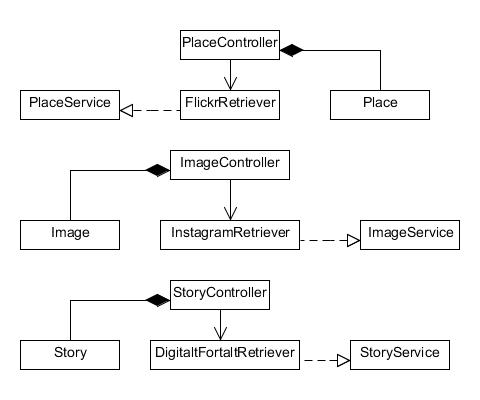
\includegraphics[width=0.8\textwidth]{Figures/Architecture/serverLogical.jpg}
      \caption{Server - Logical view}
      \label{fig:arch_server_logical}
\end{figure}

\subsubsection{Process view}
The process in the server is quite simple as it is modeled on the way HTTP works, and the way browsers threats HTML. The client sends a request to an URL and the Play! Frameworks main controller delegates the  responsibility of delivering data to the correct controller based on the URL requested. If the content received has connections to other types of content on the server, the client will have to send a new request for that content.

\begin{figure}[H]
      \centering
      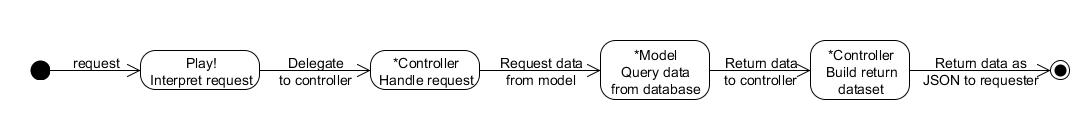
\includegraphics[width=0.8\textwidth]{Figures/Architecture/serverProcess.jpg}
      \caption{Server - Process view}
      \label{fig:arch_server_process}
\end{figure}

Note that *Controller and *Model means every corresponding pair of models and controllers.

\subsubsection{Development view}
DATABASE represents all the data. In this layer the work of structuring the data and figuring out the database design is also included.

MODELS represents the classes that will be used to work with the database from the rest of the backend code. The models will abstract away the database, so that it can be changed in its entirety if needed without changing any other code.

CONTROLLERS represents the classes that handles the requests and returns data to the client or sends it to the model for storage in the database.

\begin{figure}[H]
      \centering
      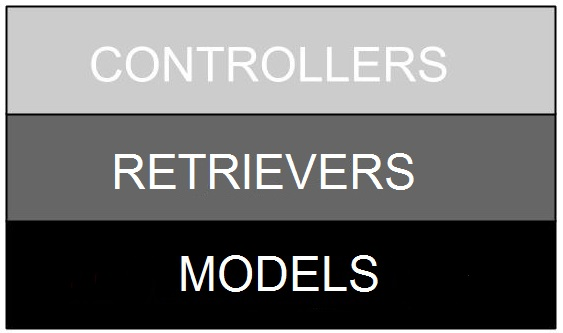
\includegraphics[width=0.8\textwidth]{Figures/Architecture/serverDevelopment.jpg}
      \caption{Server - Development view}
      \label{fig:arch_server_development}
\end{figure}

\subsection{Client}

\subsubsection{Logical view}

\subsubsection{Process view}

\subsubsection{Development view}

\section{Architectural rationale}

\chapter{Testing}

\section{Test plan}

The items and the form and content of the each test document is based on the IEEE Standard 829 \cite{ieee829}. So according to the definition of test plan in the standard: ``The test plan prescribes the scope, approach, resources, and schedule of the testing activities. It identifies the items to be tested, the features to be tested, the testing tasks to be performed, the personnel responsible for each task, and the risks associated with the plan''.

\subsection{Test plan identifier}
Let this test plan to be identified as ``VirtualWall\_TESTPLAN\_1''.

\subsection{Introduction}
The Virtual Wall software system consists of two subsystems:

\begin{itemize}
	\item backend/server
	\item frontend/client (mobile/web application)
\end{itemize}

The backend is the part of the system where all the data is stored. The backend serves the clients with the data on demand.

The client is the part of the system that presents the data to the user and that directly interacts with the user.

\subsection{Test items}
Following items thall be tested:

\begin{itemize}
	\item The source code of server subsystems will be tested.
	\item The source code of client subsystems will be tested.
	\item The user interface of the client subsystem will be tested.
\end{itemize}

\subsection{Features to be tested} \label{sec:test_plan_features_tested}
All functional requirements listed in \ref{chap:req} for this project shall be tested, unless listed as features not to be tested under \ref{sec:test_plan_features_not_tested}.

\subsection{Features not to be tested} \label{sec:test_plan_features_not_tested}
There are no items known not to be tested.

\subsection{Approach}
The overall approach is to perform a system test of all features listed under \ref{sec:test_plan_features_tested} using tests cases specified in \ref{sec:test_cases}.

During the development, the source code shall be tested using unit tests prepared by developers themselves. This simplifies the integration by making problems to be found early.

Resulting source code of both subsystems shall be tested using black-box testing. This enables us to abstract from the source code and only focus on the output and outcomes of actions, and compare this with the expected results. These tests are going to be based on test cases specified below and will be performed by black-box testers.

Apart from black-box testing, we shall perform a code inspection to assure desired quality attributes (listed in \ref{sec:architecture_drivers}) such as modifiability. This shall be done by white-box testers, i.e. members of the development team themselves.

All testing shall be done according to the time plan specified in the schedule table below.

Testing of the user interface shall be done by intended users of the system by means of usability testing. %FIXME SIMON: TBD usability testing

\subsection{Item pass and fail criteria}
Meeting the preconditions for each test and receiving a corresponding expected result are criteria for successful passing the test. The test is evaluated as failed otherwise.

%FIXME SIMON: TBD
%\subsection{Suspension criteria and resumption requirements}

\subsection{Test deliverables}
The documents to be delivered shall include:

\begin{itemize}
	\item SRS (System Requirements Specification)
	\item Test procedures specification (test cases)
	\item Test logs (test results)
	\item Test summary report (evaluation)
\end{itemize}

\subsection{Environmental needs}
Backend subsystem shall be deployed on a server running JRE 1.6 and an instance of PostgreSQL database. The database needs to contain specified schema with structure according to DDL scripts.

Server computer needs to be connected to the Internet. Specified port shall be open for server to listen on and reachable from outer network (not blocked by a firewall, etc). %FIXME SIMON: mention port number once it's known

Device to run the client needs to be equipped with a web browser to open the web application in. The device needs to be connected to the Internet.

\subsection{Responsibles}

The table \ref{tab:test_plan_tasks_allocation} maps responsibilities to roles in the scope of testing.

\begin{table}[H]
	\centering
	\begin{tabular}{| l | l |}
		\hline
		Task 				& Responsible role 	\\ \hline

		Test management 	& test manager 		\\ \hline
		
		Test design 		& test developers 	\\
							& test manager 		\\ \hline
		
		Test preparation 	& white-box testers \\
							& test manager 		\\ \hline
		
		Test execution 		& white-box testers \\
							& black-box testers \\
							& usability testers \\ \hline
		
		Test evaluation 	& test manager 		\\ \hline
	\end{tabular}
	\label{tab:test_plan_tasks_allocation}
	\caption{Roles allocation for testing tasks.}
\end{table}

The table \ref{tab:test_plan_roles_allocation} maps roles in testing to the members of the development team.

\begin{table}[H]
	\centering
	\begin{tabular}{| l | l |}
		\hline
		Role 				& Names of allocated persons 	\\ \hline

		Test manager 		& Simon Stastny 				\\ \hline

		Test developers 	& Christian Frøystad 			\\
							& Odd Fredrik Rogstad 			\\
							& Knut Nergård 					\\
							& Simon Stastny 				\\ \hline

		White-box Testers 	& Christian Frøystad 			\\
							& Odd Fredrik Rogstad 			\\
							& Knut Nergård 					\\
							& Simon Stastny 				\\ \hline

		Black-box Testers 	& TBD 							\\ \hline %FIXME SIMON: determine black-box testers

		Usability Testers 	& TBD 							\\ \hline %FIXME SIMON: determine usability testers
	\end{tabular}
	\label{tab:test_plan_roles_allocation}
	\caption{Roles allocation for testing tasks.}
\end{table}

\subsection{Staffing and training needs}
For blackbox testing, the test responsible needs to be instructed about the system workflow in order to be able to follow the steps listed in the test cases.

For code inspection, the person performing it must have a detailed knowledge about the inner workings of the system to be able to discover possible problems and/or draw up improvements of the current solution.

For usability testing, the tester shall have (in the direction of this system) no further knowledge than what is expected to be a minimum knowledge needed for the end user to use the software . This typically includes user knowledge of computer/smartphone/tablet operations and interaction with the device (direct pointing, keyboard, or some characteristic touch gestures). Tester especially should not have an a priori knowledge about the system workflow, since this is something a typical end user will not have.
\subsection{Schedule}

The table \ref{tab:test_plan_schedule} lists tasks and maps them to people responsible for them and dates due to which they should be finished. 

\begin{table}[H]
	\centering
	\begin{tabular}{| l | l | l |}
		\hline
		Task 								& Responsible 	& Due date		\\ \hline
		Design test cases for system tests 	& Simon Stastny & 2013-10-31 	\\ \hline
		Design usability tests 				& TBD 			& TBD 			\\ \hline
		Perform black-box tests 			& TBD 			& TBD 			\\ \hline
		Perform usability tests 			& TBD 			& TBD 			\\ \hline
	\end{tabular}
	\label{tab:test_plan_schedule}
	\caption{Test tasks schedule}
\end{table}

In case the functional requirements are a subject to change in the future, the design of black box tests may get delayed to absorb the changes in the requirements specification. The black box test design can only be as much finished as the functional requirement specification is.

\subsection{Risks and contingencies}

As far as we are aware, there are no risks related to testing but those mentioned in \ref{sec:project_risk_assessment} as general risks for this project.

\subsection{Approvals}

The table \ref{tab:test_plan_approvals} lists approvals of completed tasks.

\begin{table}[H]
	\centering
	\begin{tabular}{| l | l | l |}
		\hline
		Task 								& Approved by 	& Date 	\\ \hline
		Design test cases for system tests 	& Simon Stastny & 		\\ \hline
		Design usability tests 				& 				& 		\\ \hline
		Perform black-box tests 			& 				& 		\\ \hline
		Perform usability tests 			& 				& 		\\ \hline
	\end{tabular}
	\label{tab:test_plan_approvals}
	\caption{Test tasks approvals}
\end{table}

\section{Test cases} \label{sec:test_cases}

\section{Test results and evaluation}

\chapter{Phases}
\section{Planning}

\section{Sprint 1}
\subsection{S1: Introduction}
The aim of this first sprint is to establish a baseline, in terms of technology but also with regard to the social aspects of executing a sprint as well as the amount of work being manageable within the timespan of the sprint.

\subsection{S1: Requirements}
The server as well as the client should have a base satisfying the architectural drivers listed in \ref{sec:architecture_drivers}.

\subsection{S1: Pre study}

\subsubsection{Server}
This is the pre study done for the server in sprint 1.

\textbf{Extensible Markup Language (XML) vs JavaScript Object Notation (JSON)}\\
XML is a extensible markup language created by the World Wide Web Consortium (W3C). It is made to be both human and machine readable. It consists of a developer defined set of nested elements that may contain data or new elements.

JSON \cite{json} is based on two structures: a collection of name-value pairs, and an ordered list of values. The format is made to be human readable and easily parsed and created by computers. It is based on a subset of the JavaScript programming language, and because the customer has asked for HTML5 to be used for the app JSON makes sense as that will be easier to use together with JavaScript than XML.

\textbf{Representational State Transfer (REST) vs Simple Object Access Protocol (SOAP)}\\
REST \cite{rest} is an architectural style that is stateless at its heart, which leads to better visibility, reliability, and scalability. REST was developed in parallel with HTTP/1.1 and the largest system following this architectural style is the internet (according to \cite{wikipedia:rest}). REST is also a good match for data driven applications as the way you handle a REST services is by utilizing the verbs GET, POST, DELETE, PUT, PATCH.

SOAP is much more flexible than REST, but also much more complex. While REST is primarily data driven through resources, SOAP is logic oriented through operations. SOAP is also a better choice for making stateful web services. All communication with a SOAP service happens through XML.

The simplicity of the REST architectural style, and the fact that it allows the developer to choose the format of exchange makes this our preferred way to go.

\textbf{Play vs Spring}\\
Two of the well known frameworks when it comes to developing webservices in JAVA is Play! Framework and Spring.

Spring is a very extensive framework with support for quite a few protocols and services. The framework also does a lot of work not necessarily apparent to the developer without a thorough investigation into the documentation.

The Play! Framework is more of a core framework that does the basics, but leaves it to the developer to develop the application in mostly his own style. Different from Spring, Play! Framework also reloads automatically every time a change occurs in the source, and in this way contributes to more effective development.

The extensive documentation and speed of development made us choose Play! Framework for the system.

\textbf{MySQL vs Postgres}\\
The database system most known to the developers is MySQL as this has been used in several earlier courses. Both systems are highly capable relational databases with good coverage of features and excellent performance. There are, however, particularly one issue that separates them, and make one stand out as our database of choice.

In April 2009 Oracle bought Sun \cite{sun}, and by that gained control of MySQL. Initially Oracle promised that MySQL would prevail and that it and its coming features would stay open source \cite{mysql}. The situation today shows that they have not honored that promise, and several different versions of MySQL are availiable \cite{mysqlproducts}. This serves to show that the future of MySQL is uncertain, and as such our choice falls on Postgres.

\subsubsection{Client}
The client requested use of HTML5 on the client side, so that the prototype could be tested by the whole of the test group without having to hand out phones of a specific type, but rather let the test objects use their own devices.

When it comes to real cross platform HTML5 apps, that is to say no need for native code at all, Apache Cordova is a very useful project. Apache Cordova is what was earlier known as PhoneGap \cite{phonegap}. The code was contributed to The Apache Software Foundation in 2011, at the same time Adobe acquired PhoneGaps creators Nitobi.

The way Cordova works is that it exposes native interfaces through JavaScript libraries, so that local web clients might use native features like gyroscope, accelerometer, etc. When the application is built using web technologies, it is compiled into a native webcontainer. In order to do this, one needs to have access to the platform one compiles for. For Android, you need the Android SDK. For iOS, you need an Apple computer and Xcode. For Blackberry you need WebWorks SDK.

The need for all this different platforms when building defies some of the intention of using a cross platform framework for developing the app, as it would make the workload and expenses grow quite substantially.

This is where Intel XDK comes in handy. It is a simple IDE for native web apps development with Cordova. It also includes an emulator, so that testing across units is much simplified. When ready to test on phones or build final version for deployment, Intel provides building for all platforms with a simple click in interface.

Intel also provides a fast and native looking HTML5, JavaScript and CSS library with their XDK, but due to very poor documentation for systems wishing to retain the qualities of modifiability and maintainability, the library was rejected.

Investigation into best fitted client side framework will continue into the next sprint.

\subsubsection{Interaction and user interface}
When the sprint started it was quite unclear how the application would look and feel. Within this sprint there has been two iterations on the user interface.

\textbf{Version one}\\
First thing done was to come up with what kind of main functionality the application needed;

\begin{itemize}
	\item Some kind of menu system, to navigate in the application
	\item A function to browse walls
	\item A way of displaying walls and stories
\end{itemize}

Another concern was about the definition of a wall and story, thus what kind of information did it need to display.

\textit{Menu}\\
We saw two opportunities, a dedicated menu, typically the start up point for the application, and a more hidden menu, that we'll refer to as a side-menu. The dedicated menu is typically made up with buttons, where the user can access all top-level functions. It is easy and straightforward to implement, it is also well known for most users. A more elegant solution is the hidden side-menu, where the user can access the menu wherever he or she is in the application, with just a sliding gesture from right to left on the screen.

\begin{figure}[H]
    \centering
    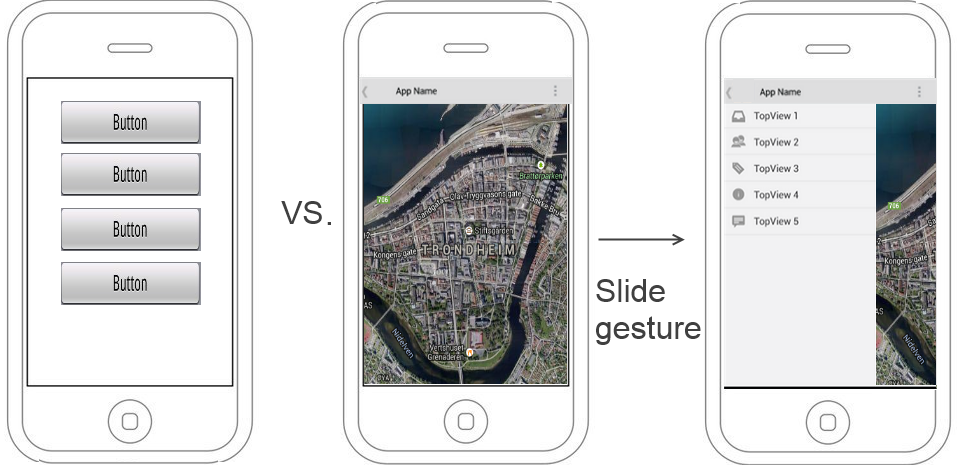
\includegraphics[width=0.8\textwidth]{Figures/Phases/Sprint1/versiononeSliding.png}
    \caption{Menus, dedicated vs. hidden side-menu}
    \label{fig:phases_sprint1_uiVersionOneMenu}
\end{figure}

The customer prefered the hidden side menu.

\textit{Browsing walls}\\
An important function is to let the user browse and find walls. The most obvious solutions, to use a map and/or a list, were discussed, but no solution was determined. 

Another important function is to filter or sort the walls. In a list it is easy to sort the walls on, for instance, popularity or the distance to your location using GPS tracking. There were suggested to use some kind of temperature pins in a map, where the pins shows the user how popular the different places are by using colors. The user could also decide to only see the most popular places by excluding the more cold colored walls, as Figure~\ref{fig:phases_sprint1_uiVersionOneTempPings} shows. The temperature pins were just one of many suggestion on how to represent walls on a map, others where to use symbols or icons, one colored pins and images.

The customer wanted to focus more on the use of filtering on tags and metadata.

\begin{figure}[H]
    \centering
    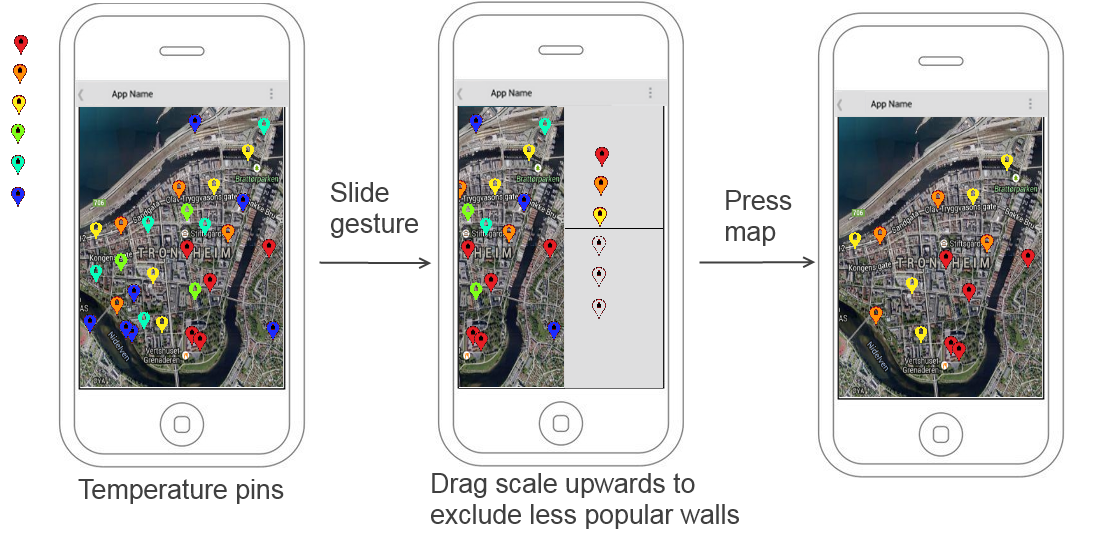
\includegraphics[width=0.8\textwidth]{Figures/Phases/Sprint1/versiononeTempPings.png}
    \caption{Temperature pins, with filtering}
    \label{fig:phases_sprint1_uiVersionOneTempPings}
\end{figure}

\textit{Look at walls}
The main function of the application is to access a wall and browse user created information, that could be stories, pictures, links to other resources, etc.. Two possible solution were suggested; a wall that displayed both user created stories and information from multiple data sources as in Figure~\ref{fig:phases_sprint1_uiVersionOneSimpleWall}, for instance, Instagram, Wikipedia, YouTube, Twitter, Google, Flickr, etc., and a more simple version where the focus was on user created data, thus stories and pictures, as in Figure~\ref{fig:phases_sprint1_uiVersionOneMultipleDataSoruces}.

The idea of using multiple data sources came from the danish mobile application, Kulturarv, or Cultural Heritage (both mentioned in \ref{sec:prestudy_existing_apps}), which blends data from a main database with other geo location data sources like Instagram, Flickr, Wikipedia and Twitter. The customer had not thought about the idea of using multiple data sources, and were therefore quite surprised by the solution. The group and customer agreed that the use of multiple data sources were out of the scope, and decided to focus on the more simple version.

\begin{figure}[H]
    \centering
    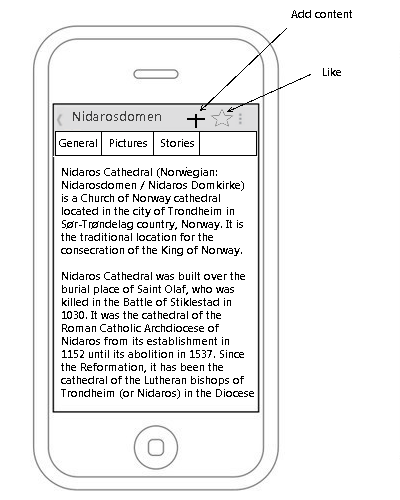
\includegraphics[width=0.8\textwidth]{Figures/Phases/Sprint1/versiononeSimpleWall.png}
    \caption{Simple wall, with tabs to navigate. Nidarosdomen is used as an example}
    \label{fig:phases_sprint1_uiVersionOneSimpleWall}
\end{figure}

\begin{figure}[H]
    \centering
    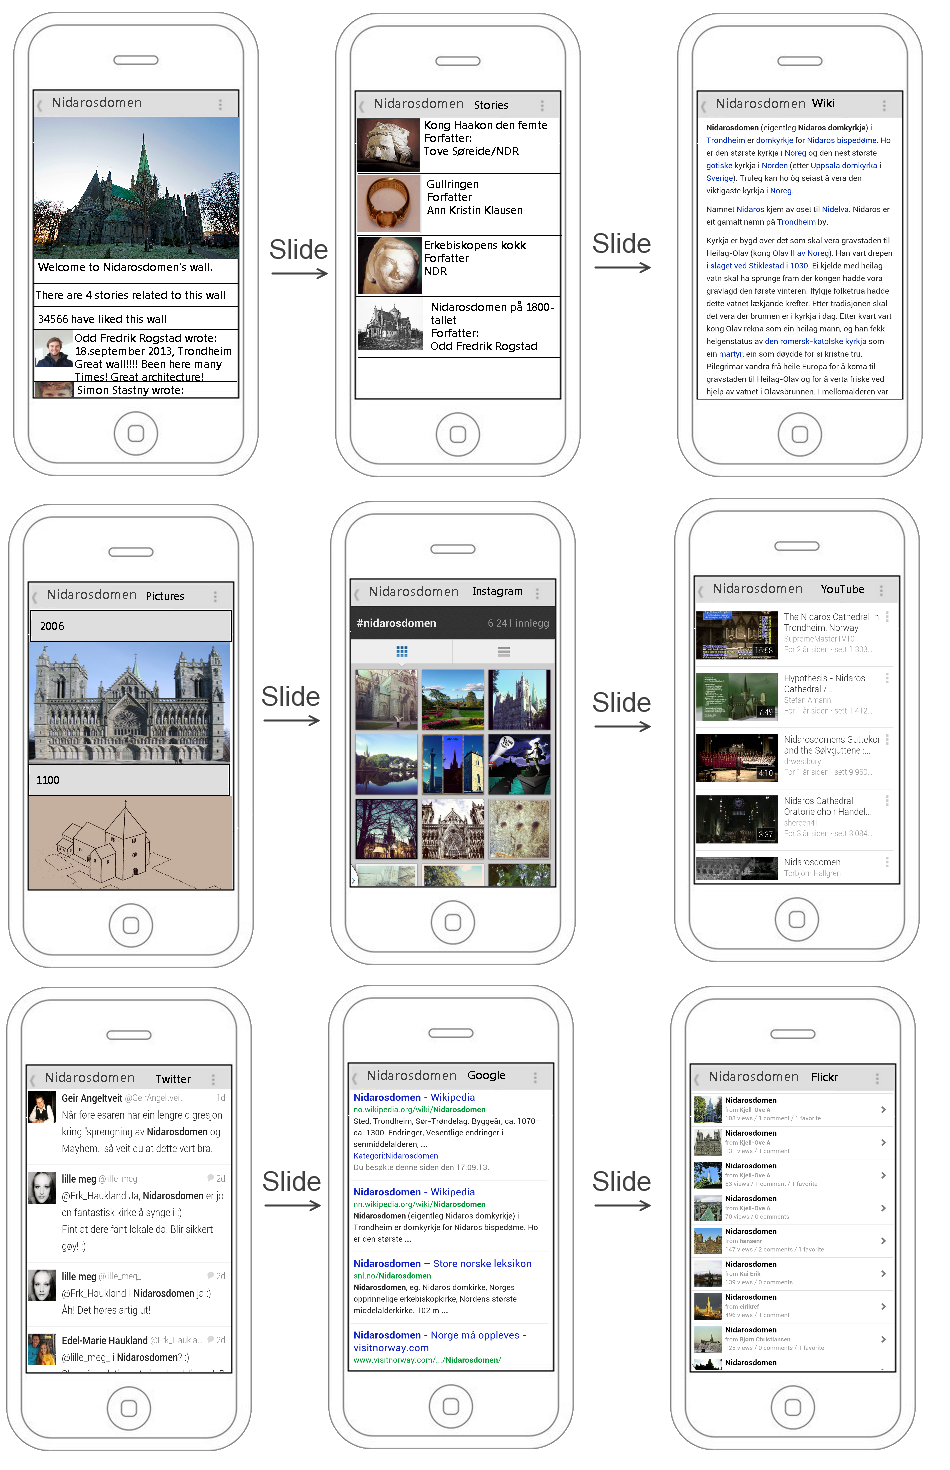
\includegraphics[width=0.8\textwidth]{Figures/Phases/Sprint1/versiononeMultipleDataSourcesWall2.png}
    \caption{Wall using multiple data sources, with slide gestures to navigate. Nidarosdomen is used as an example}
    \label{fig:phases_sprint1_uiVersionOneMultipleDataSoruces}
\end{figure}

\textbf{Version two}\\
TBA

\subsection{S1: Implementation}

\subsubsection{Server}
During this period only the most basic proof of concept was developed for the server. A RESTful access point was made for the developed, with a database. All the basic groundwork was put in place, except for authentication, to develop the rest of the service.

\subsection{S1: Testing}
This sprint no formal testing was done, only functional tests on the server and discussions around the user interface.

\subsection{S1: Review}
We did not manage to finish all the predefined tasks for this sprint. This was partly due to the absence of two group members during most of the sprint period. The delay was also partly due to inexperience with mobile JavaScript frameworks and the lack of real documentation for most of them.

\section{Sprint 2}
\subsection{S2: Introduction}
The goal of the second sprint was initially to build upon the bases put in place by sprint one, but due to a steep learning curve in JavaScript and lack of real documentation for most frameworks this was not the case.

The server has seen development based upon what was done in sprint one, but the client has started from scratch.

\subsection{S2: Backlog}
\begin{table}[H]
	\centering
	\begin{tabular}{| l | l |}
		\hline
		Item 				& Outcome\\
		\hline
		Define the concept of story & Done\\
		\hline
		Define the main principles of UI & Done\\
		\hline
		Browse virtual walls & Done in server\\
		\hline
		Open a virtual wall & Done in server\\
		\hline
		Basic framework for app with support for communicating with server & Done\\
		\hline
		Architecture & Partly done\\
		\hline
	\end{tabular}
	\label{tab:phase_sprint2_backlog}
	\caption{Backlog for sprint 2.}
\end{table}

\subsection{S2: Requirements}

\subsection{S2: Pre study}

\subsubsection{Client}

\textbf{The M project}\\
Initially “The M project” \footnote{http://www.the-m-project.org/} came out quite good in comparisons of frameworks for client side development for mobile phones. This was due to it being lightweight and what seemed like usable documentation. Its described caracteristica also matched quite good with what we was looking for. Especially the MVC part and the native look and feel of the jQuery Mobile user interface. The MIT license was also very attractive, as it is compatible with the BSD license required for all code produced in this course.

The reasons why The M project was not chosen in the end, surrounds two topics. First, the project has its own build system to help the developers develop more efficiently. Unfortunately this did not work, and produced unrunnable code. One could edit the files after each build in order to make them runnable, but 5 minutes extra per build to clean the code was just not acceptable.

The second problem is of a more serious kind, both for this development team and for those that might follow at a later time. The documentation was vague at best and partly outdated.

\textbf{Enyo}\\
Enyo\footnote{http://enyojs.com/} was developed by HP for WebOS\cite{enyoHistory} and is at this time sponsored by LG. It has a very interesting approach to development, one develops features in the app as separate reusable components and glue them together. In that way it feels much more natural to develop in Enyo, and the documentation is excellent. The license, Apache 2.0, is also very attractive as it is compatible with BSD.

The problem with Enyo was that the requirements specified modifiability as one very important factor to take into account. While components can make the app itself modifiable, Enyo does not support MVC in the components and as such one just moves the complexity one level down. When developing components we would still have to handle that lack of ability to structure the code in an efficient way.

Adding support for MVC, or making it easy to use MVC in combination with the rest of the framework, is an ongoing effort at Enyo.

The reason Enyo was not selected is that the MVC support has not yet stabilized, and the documentation is still a bit too thin on the matter.

\textbf{Sencha Touch}\\
Sencha Touch\footnote{http://www.sencha.com/products/touch/} has excellent documentation and a good community. The problem with Sencha is the incompatible license. Sencha uses the General Public License version 3, which is incompatible with the BSD license.\cite{flossLicense}

\textbf{RhoMobile}\\
RhoMobile is developed by Motorola Solutions\footnote{http://www.motorolasolutions.com/US-EN/Business+Product+and+Services/Software+and+Applications/RhoMobile+Suite} to help developers develop software across their different handheld devices. They have also added support for the mobile platforms. This framework has support for developing enterprise applications and has an attractive license in MIT.
The reason this framework was not chosen, was because it uses Ruby as well as JavaScript. It was decided that learning one new language would be enough work, if not another one should be added on top.

\textbf{Titanium}\\
Appcelerator Titanium\footnote{http://www.appcelerator.com/titanium/} is a cross platform development framework for mobile and web. The development is done in JavaScript and XML. It is licensed under the Apache Public License version 2. Titanium is a "write once, adapt everywhere" framework\cite{titaniumCrossMobile}. That does not mean that it can’t run everywhere without adaption, but that in order to look native it needs adaption. Titanium has an excellent base of documentation and a mature framework supporting easy use of the model view controller architectural pattern.

Titanium was chosen because of its framework, its documentation and the huge community that surrounds it.


\subsection{S2: Implementation}

\subsubsection{Server}

In this sprint the requirements for the overall workings of the system seemed to be somewhat stable so we designed a data model and implemented it on the server side. This turned out to be a wrong assumption later on.

\subsubsection{Client}
\textbf{Sync client}\\
Titanium Alloy is backend agnostic. This means that most of the code does not know, nor need to know, what kind of backend is running. This is accomplished by utilizing an abstraction layer in Alloy called Sync. Sync provides an unified API that can be implemented for each type of backend.\\
The API has the following methods:

\begin{table}[H]
	\centering
	\begin{tabular}{| l | l | l | l |}
		\hline
		Backbone Method & Sync CRUD Method & Equivalent HTTP Method & Equivalent SQL Method\\
		\hline
		Collection.fetch & read & GET & SELECT\\
		\hline
		Collection.create (id == null) or Collection.create (id != null) & create or update & POST or PUT & INSERT or UPDATE\\
		\hline
		Model.fetch & read	& GET & SELECT\\
		\hline
		Model.save (id == null) or Model.save (id != null) & create or update & POST or PUT & INSERT or UPDATE\\
		\hline
		Model.destroy & delete & DELETE & DELETE\\
		\hline
	\end{tabular}
	\label{tab:phase_sprint2_model}
	\caption{API for Sync in Alloy\cite{titaniumAlloySync}}
\end{table}

As the application makes use of REST server, a backend supporting REST was needed. Although a custom backend could have been created, it made more sense to reuse the implementation of others. The napp.alloy.adapter.restapi\footnote{https://github.com/viezel/napp.alloy.adapter.restapi} by Mads Møller was chosen due to its feature completeness and active development.

\textbf{Models}\\
Models in Titanium Alloy build upon Backbone.js\footnote{http://backbonejs.org/} \cite{titaniumAlloyModel}. Therefor the documentation for Backbone.js is relevant in addition to the documentation from Titanium.

A basic model looks like this:
\begin{lstlisting}
exports.definition = {
        config : {
                "columns"        : {
                        "wallId"                 : "int",
                        "name"     	     : "string",
                        "description"         : "string",
                        "latitude"               : "double",
                        "longitude"            : "double",
                },
                "URL"           : "http://stedr.herokuapp.com/walls.json",
                "adapter"      : {
                        "type"        : "restapi",
                        "collection_name" : "wall",
                        "idAttribute" : "wallId"
                }
        },
        extendModel : function(Model) {
                _.extend(Model.prototype, {
                        // If adding and editing walls shall be allowed, the specific url must be added here
                });
                return Model;
        },
        extendCollection : function(Collection) {
                _.extend(Collection.prototype, {});
                return Collection;
        }
};
\end{lstlisting}

\subsection{S2: Testing}
Only functional testing was done for this sprint as development went on. No systematic testing was executed.

\subsection{S2: Review}
Once again we would like to have reached a milestone farther ahead at this time, but we have had to spend a lot more time learning new mobile frameworks than we had expected. 

Nevertheless, the group has seen increased participation during this sprint, and more group members has become more active. This has lead to us getting more done than in the earlier sprints, and we how this will also mean that we will get even more done in the coming sprints.

Some of our goals for this sprint was only reached for the server. The reason for this is the fact that the group members are more accustomed to Java than JavaScript, and the fact that Play! Framework has better documentation available than the mobile frameworks we have used.

The architecture is only partially done, this is due to the change in mobile framework and requirements. Now that a mobile framework has been chosen and the requirements more stabilized, we hope to have the architecture finished within a relatively short amount of time.

\section{Sprint 3}
\subsection{S3: Introduction}
\subsection{S3: Requirements}

\subsection{S3: Pre study}

\subsubsection{Map views, coordinates and projections} \label{sec:spr3_maps}

One of the main features of the application is to show user location of various virtual walls on a map. Since we decided to use Titanium frameworkk for the development of the mobile application, we are using its own map view (\texttt{Titanium.Map.View}) for the display of maps and locations of walls upon them.

The database is now featuring just a few walls, but it is supposed to host much more of them in the future and it would not be optimal for the performance and operational reasons (such as costs of data transfers on mobil internet) to fetch all the walls when user is using the application.

The user is only interested in walls he could actually see on the map, so we decided to take an approach where we fetch the data from the server while filtering it upon geographic coordinates. The map view supplies us with a geogaphical coordinates of the center of the displayed map and with west-to-east distance and noth-to-south distance. This makes it possible to compute the coordinates of the north-west (i.e. top-left) corner of the map view, and the south-east (i.e. bottom-right) corner of the map view. Then the application fetches the data from the server, asking it to filter only those walls, which have coordinates in the rectange defined by those two corners.

It is a well-known fact that planet Earth is not flat. For this reason, various map projections are used to transform the surface of Earth (3D) onto a plane (2D). Google Maps, which provide the map tiles for the map view, are using a variant of so called Mercator \footnote{Named after Flemish geographer and cartographer Gerardus Mercator, who firstly used it in 1569 for his map titled \emph{Nova et Aucta Orbis Terrae Descriptio ad Usum Navigantium Emendate Accommodata}, which is Latin for \emph{New and more complete representation of the terrestrial globe properly adapted for use in navigation}.} projection. This map projection was used in naval navigation for showing constant bearings (\emph{loxodromes}, also known as \emph{rhumb lines}) as straight lines on the map. \cite{progonos:mercator,radicalcartography} 

\begin{figure}[H]
    \centering
    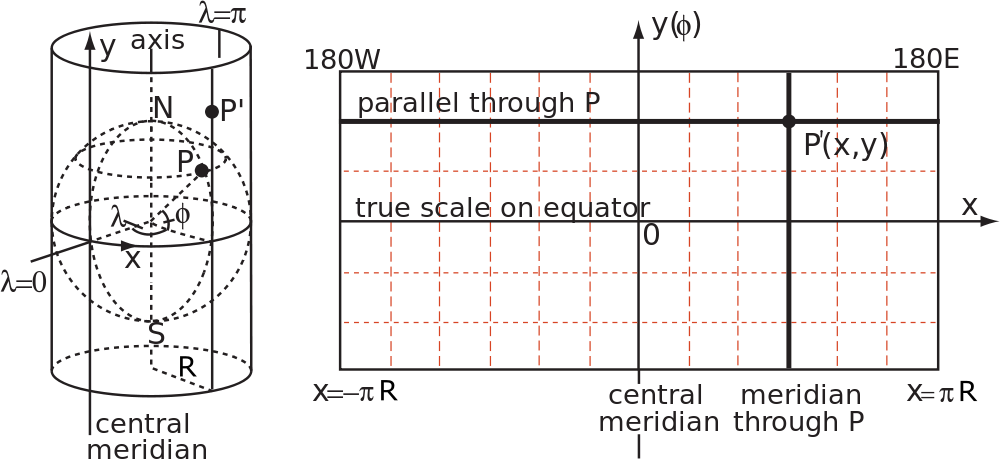
\includegraphics[width=0.8\textwidth]{Figures/Prestudy/mercator.png}
    \caption{Mercator cylindrical map projection basics. \cite{wikipedia:mercator}}
    \label{fig:mercator}
\end{figure}

As seen in \ref{fig:mercator}, it is a cylindrical conformal projection, so it preserves local angles (which is actually one of the reasons Google Maps use it), but is unfit for use in high-latitudes as the map extends infinitely North and South (so called \emph{polar exaggeration}). This shall be fine for use until we need to add a wall for a location near to one of the geographic poles (which are streched infinitely along the top and bottom edges of the map). This could be a problem is we want to add a wall for example for the Amundsen–Scott South Pole Station located just few meters from the geographical souch pole and which would and stretch widely east to west. \cite{progonos:mercator,radicalcartography} 

\subsection{S3: Implementation}

\subsubsection{Server}

Upon receiving changes proposed by customer, the data model was stashed and reworked to acomodate the proposed changes. As the concept of walls and stories finally settled down, we were able to implement API for retrieving walls based on geographic coordinates and to retrieve stories on walls.

As requested in the last batch of change requests from customer, stories shall be stored in an external database called \emph{Digitalt Fortalt}. This database provides an API for search which we call to retrieve the stories. Our application does not write any data to \emph{Digitalt Fortalt}, stories need to be created manually on their website.

Walls on the other hand shall be stored in out system database. We now store each wall with its geographic coordinates in a database table and filter as described in \ref{sec:spr3_maps}. 

Data stored in our database are retrieved by classes in the \texttt{models} package. The models are extending \texttt{play.db.ebean.Model} class and use standard JPA\footnote{Java Persistence API} annotations to indicate relationships between entities.

The data from \emph{Digitalt Fortalt} are retrieved from the API by classes in the \texttt{retrievers} package. The data are fetched and parsed by using the \emph{jsoup} Java HTML parser. We found this library to be more usable than \emph{DOM} and \emph{SAX} parser implementations in Java (due to various reasons such as usage of \texttt{Iterable} interface, which make the work with collection-like structures much easier).

\subsection{S3: Testing}
\subsection{S3: Review}
\subsection{S3: Phase evaluation}

\section{Sprint 4}
\subsection{S4: Introduction}
\subsection{S4: Requirements}
\subsection{S4: Pre study}
\subsection{S4: Implementation}
\subsection{S4: Testing}
\subsection{S4: Review}
\subsection{S4: Phase evaluation}

\section{Finalization}
\subsection{F: Introduction}
\subsection{F: Requirements}
\subsection{F: Pre study}
\subsection{F: Implementation}
\subsection{F: Testing}
\subsection{F: Review}
\subsection{F: Phase evaluation}



\chapter{Evaluation}

\bibliography{bibliography}

\appendix
\chapter{Assignment}

\chapter{Timesheets}

\chapter{Documentation}

\end{document}